\documentclass{article}
\usepackage{amsmath,amsxtra,amssymb,latexsym, amscd,amsthm}
\usepackage{indentfirst}
\usepackage[mathscr]{eucal}
\usepackage[utf8]{vietnam}
\usepackage{indentfirst}
\usepackage{array}
\usepackage{setspace}
\usepackage{graphicx}
\usepackage{xhfill}
\usepackage[left=2cm,right=2cm,top=2cm,bottom=2cm]{geometry}

\setlength{\parindent}{5pt}
\begin{document}
\newcommand{\xfill}[2][1ex]{{%
  \dimen0=#2\advance\dimen0 by #1
  \leaders\hrule height \dimen0 depth -#1\hfill%
}}

%Cover
\begin{center}
    
    \fontsize{14pt} {20pt}\selectfont
    \textsc{TỔNG LIÊN ĐOÀN LAO ĐỘNG VIỆT NAM\\}
    \textbf{TRƯỜNG ĐẠI HỌC TÔN DỨC THẮNG\\}
    \textbf{KHOA CÔNG NGHỆ THÔNG TIN\\}
    \vspace{1 cm}
    
        \begin{figure}[htp]
            \centering
           
\includegraphics{2.jpg}
        \end{figure}
     
     
     
    \fontsize{16}{20}\selectfont\textbf{ĐỒ ÁN CUỐI KHÓA:\\}
    \fontsize{16}{20}\selectfont\textbf{MÔN PHÁT TRIỂN HỆ THỐNG THÔNG TIN DOANH NGHIỆP\\}
    \vspace{0.5CM}
    
    \fontsize{24}{20}\selectfont\textsc{PHÂN TÍCH VÀ THIẾT KẾ\\ CHO HỆ THỐNG CỬA HÀNG \\BÁN DỤNG CỤ THỂ THAO SALOMON \\}
    \end{center}
    \vspace{2cm}
    \begin{flushright}
       \setstretch{1}
        \fontsize{14}{20}\selectfont
        \textit{Người hướng dẫn}: \textbf{Giảng viên Dương Hữu Phúc}\\
        \textit{Người thực hiện}: \textbf{Đào Hữu Hoàng Quân - 51703164}\\
        \textbf{Nguyễn Thế Anh Khoa - 51703114}\\
         \textbf{Lê Thành Kiến An - 51703037}\\
    \end{flushright}
    \vspace{3cm}
    \begin{center}
     \fontsize{14}{20}\selectfont
   \textbf{THÀNH PHỐ HỒ CHÍ MINH,NĂM 2019}
\end{center}
%%SubCover
\pagenumbering{gobble}
\begin{center}
    \pagenumbering{gobble}
    \fontsize{14pt} {20pt}\selectfont
    \textsc{TỔNG LIÊN ĐOÀN LAO ĐỘNG VIỆT NAM\\}
    \textbf{TRƯỜNG ĐẠI HỌC TÔN DỨC THẮNG\\}
    \textbf{KHOA CÔNG NGHỆ THÔNG TIN\\}
    \vspace{1 cm}
    
        \begin{figure}[htp]
            \centering
           
\includegraphics{2.jpg}
        \end{figure}
     
     
     
    \fontsize{16}{20}\selectfont\textbf{ĐỒ ÁN CUỐI KHÓA:\\}
    \fontsize{16}{20}\selectfont\textbf{MÔN PHÁT TRIỂN HỆ THỐNG THÔNG TIN DOANH NGHIỆP\\}
    \vspace{0.5CM}
    
    \fontsize{24}{20}\selectfont\textsc{PHÂN TÍCH VÀ THIẾT KẾ CHO HỆ THỐNG CỦA HÀNG BÁN DỤNG CỤ THỂ THAO SALOMON \\}
    \end{center}
    \vspace{2cm}
    \begin{flushright}
       \setstretch{1}
        \fontsize{14}{20}\selectfont
        \textit{Người hướng dẫn}: \textbf{Giảng viên Dương Hữu Phúc}\\
        \textit{Người thực hiện}: \textbf{Đào Hữu Hoàng Quân - 51703164}\\
        \textbf{Nguyễn Thế Anh Khoa - 51703114}\\
         \textbf{Lê Thành Kiến An - 51703037}\\
    \end{flushright}
    \vspace{3cm}
    \begin{center}
     \fontsize{14}{20}\selectfont
   \textbf{THÀNH PHỐ HỒ CHÍ MINH,NĂM 2019}
\end{center}
% Loi_cam-on

\begin{center}
    \fontsize{16}{20}\selectfont
    \textbf{LỜI CẢM ƠN\\}
\end{center}
    \fontsize{14}{20}\selectfont
    \setlength{\parindent}{1cm} 

Cảm ơn thầy Dương Hữu Phúc đã hỗ
trợ nhóm chúng em trong việc lựa chọn đề tài và hỗ trợ chúng em trong khi thực hiện đồ án.Tuy có những sai sót, mong thầy cô phản hồi và đưa ra phương án giúp chúng em khắc phục.Chúng em xin cảm ơn!!!
\setcounter{page}{1}
\pagenumbering{arabic}
\pagebreak
%Loi_cam_ket
\begin{center}
    \fontsize{16}{20}\selectfont
    \textbf{ĐỒ ÁN ĐƯỢC HOÀN THÀNH\\}
    \textbf{TẠI TRƯỜNG ĐẠI HỌC TÔN ĐỨC THẮNG}
\end{center}
\fontsize{14}{20}\selectfont

Tôi xin cam đoan ây là sản phẩm đồ án của chúng tôi và được sự hướng dẫn của TS Dương Hữu Phúc. Các nội dung nghiên cứu, kết quả trong đề tài này là trung thực và chưa công bố dưới bất kỳ hình thức nào trước đây. Những số liệu trong các bảng biểu phục vụ cho việc phân tích, nhận xét, đánh giá được chính tác giả thu thập từ các nguồn khác nhau có ghi rõ trong phần tài liệu tham khảo.

Ngoài ra, trong đồ án còn sử dụng một số nhận xét, đánh giá cũng như số liệu của các tác giả khác, cơ quan tổ chức khác đều có trích dẫn và chú thích nguồn gốc.

Nếu phát hiện có bất kỳ sự gian lận nào tôi xin hoàn toàn chịu trách nhiệm về nội dung đồ án của mình. Trường đại học Tôn Đức Thắng không liên quan đến những vi phạm tác quyền, bản quyền do tôi gây ra trong quá trình thực hiện (nếu có).

\begin{flushright}
TP.Hồ Chí Minh, ngày 30 tháng 10 năm 2019\\
    Tác giả \\
    
    Nguyễn Thế Anh Khoa\\
    
    Đào Hữu Hoàng Quân\\
    
    Lê Thành Kiến An
\end{flushright}
\pagebreak
%Danh_gia
\begin{center}
    \fontsize{16}{20}\selectfont
    \textbf{PHẦN XÁC NHẬN VÀ ĐÁNH GIÁ CỦA GIẢNG VIÊN}
\end{center}
\fontsize{14}{20}

\textbf{Phần xác nhận của GV hướng dẫn}
\begin{flushright}

\ \xfill{1pt} \ 

\ \xfill{1pt} \ 

\ \xfill{1pt} \ 

\ \xfill{1pt} \ 

\ \xfill{1pt} \ 

\ \xfill{1pt} \ 

TP.Hồ Chí Minh, ngày  tháng  năm ......\\

(kí và ghi họ tên) \\[2.5cm]       
\end{flushright}


\textbf{Phần đánh giá của Gv chấm bài}
\begin{flushright}

\ \xfill{1pt} \ 

\ \xfill{1pt} \ 

\ \xfill{1pt} \ 

\ \xfill{1pt} \ 

\ \xfill{1pt} \ 

\ \xfill{1pt} \ 

TP.Hồ Chí Minh, ngày  tháng  năm ......\\

        (kí và ghi họ tên)
\end{flushright}
\pagebreak

\begin{center}
    \fontsize{16}{20}\selectfont
    \textbf{TÓM TẮT}
\end{center}
\fontsize{13}{20}\selectfont

Hệ thống của hàng phụ kiện thể thao Salomon là 1 cửa hàng mới và từng bước phát triển cạnh tranh với những của hàng trước đó. Dù là sinh sau đẻ muộn nhưng cửa hàng đã có ý tưởng làm ra 1 trang web nhằm quản lí việc bán hàng và việc quản lí kho, từ đó có thể vận hành công việc một cách trơn tru hơn và tăng tính chặt ché trong từng giai đoạn mà cửa hàng vận hành.

Nhóm em đã viết 1 trang web cho hệ thống cửa hàng Salomon, trong đó có phân đoạn: thanh toán hàng hóa khi khách mua hàng, quản lí kho nhập và kho xuất cho từng chi nhánh và cho toàn bộ hệ thống.
\pagebreak
%Muc_luc
\begin{center}
    \fontsize{16}{20}\selectfont
    \textbf{MỤC LỤC}
\end{center}
\fontsize{13}{20}\selectfont
\fontsize{14}{20}\selectfont\textbf{Chương 1: Đặc tả tóm tắt hệ thống Salomon}\xfill{1pt} \ 7 \\
\fontsize{12}{20}\selectfont\textbf{Chương 1.1: Thanh toán}\xfill{1pt} \ 7 \\
\fontsize{12}{20}\selectfont\textbf{Chương 1.2: Quản lý hóa đơn}\xfill{1pt} \ 7 \\
\fontsize{12}{20}\selectfont\textbf{Chương 1.3: Quản lý kho}\xfill{1pt} \ 8 \\
\fontsize{12}{20}\selectfont\textbf{Chương 1.4: Bảo hành}\xfill{1pt} \ 8 \\[0.5cm]
\fontsize{14}{20}\selectfont\textbf{Chương 2: Đặc tả chi tiết}\xfill{1pt} \ 10 \\
\fontsize{12}{20}\selectfont\textbf{Chương 2.1: Nghiệp vụ thanh toán}\xfill{1pt} \ 10 \\
\fontsize{12}{20}\selectfont\textbf{Chương 2.2: Quy trình quản lý hóa đơn}\xfill{1pt} \ 19 \\
\fontsize{12}{20}\selectfont\textbf{Chương 2.3: Quy trình quản lý kho}\xfill{1pt} \ 26 \\[0.5cm]
\fontsize{12}{20}\selectfont\textbf{Chương 3: Demo Project}\xfill{1pt} \ 43 \\
\fontsize{12}{20}\selectfont\textbf{Chương 3.1: Cài đặt môi trường Python}\xfill{1pt} \ 43 \\
\fontsize{12}{20}\selectfont\textbf{Chương 3.2: Cài đặt framework Django}\xfill{1pt} \ 46 \\

\pagebreak

\fontsize{16}{20}\selectfont\section{Chương 1:Đặc tả tóm tắt hệ thống Salomon }
\fontsize{13}{20}\selectfont
Cửa hàng gồm có 3 chức vụ sau: Quản lý tổng, Nhân viên bán hàng,Nhân viên kho. Đứng đầu cửa hàng và quản lý mọi mặt của cửa hàng là Quản lý tổng. Nhân viên bán hàng sẽ chỉ phụ trách công việc bán hàng tại cửa hàng và phụ trách thanh toán sản phẩm cho khách hàng. Và Nhân viên kho sẽ phụ trách việc quản lý kho sản phẩm gồm các công việc kiểm tra, cập nhật số lượng hàng tồn, quản lý việc nhập, xuất sản phẩm.
\fontsize{14}{20}\selectfont\subsection{Thanh Toán}
\fontsize{13}{20}\selectfont
Sau khi khách hàng chọn được sản phẩm, nhân viên sẽ thực hiện việc tạo hóa đơn thanh toán và nhập thông tin sản phẩm thông qua Mã của Sản phẩm hoặc Barcode của sản phẩm.Trang thanh toán sẽ hiển thị danh sách số sản phẩm được nhập vào và số tiền khách hàng phải thanh toán

Nhân viên thanh toán có thể chọn một hoặc nhiều phương thức thanh toán dựa trên yêu cầu của khách hàng. Các phương thức thanh toán gồm có 4 phương thức: Tiền mặt, Thẻ, Chuyển khoản, Thanh toán khi nhận hàng. Mục thanh toán khi nhận hàng sẽ dành cho những đơn đặt hàng online. 

Nhân viên thanh toán phải thực hiện việc nhập thông tin khách hàng gồm Tên và SDT 

Sau khi nhân viên hoàn tất việc nhập đầy đủ thông tin sản phẩm và thông tin khách hầng và kết thúc thanh toán bằng việc “done bill”, trang thanh toán sẽ gửi dữ liệu và lưu lại hóa đơn gồm thông tin hóa đơn (ngày thanh toán, thông tin sản phẩm được thanh toán, , số tiền thanh toán, chi nhánh cửa hàng ) và thông tin khách hàng, đồng thòi sẽ thực hiện cập nhật trừ đi số lượng sản phẩm trong kho cửa hàng đã được bán.

\fontsize{14}{20}\selectfont\subsection{Quản lý hóa đơn}

Quản lý hóa đơn dùng để lưu trữ tất cả các hóa đơn được thanh toán tại cả 2 chi nhánh của cửa hàng và chỉ được truy cập bởi quản lý tổng. Các hóa đơn trên hệ thống được tìm kiếm và truy xuất dựa trên ID khách hàng, chi nhánh cửa hàng, ngày thanh toán, sản phẩm thanh toán. 

Hệ thống quản lý hóa đơn chỉ được truy cập bởi quản lý cửa hàng. Quản lý cửa hàng có thể chỉnh sửa thay đổi, xóa hóa đơn mới trong hệ thong quản lý hóa đơn và thống kê lại các hóa đơn của tháng(Vd: tháng này bán được bao nhiêu sản phẩm tên xyz, tổng doanh thu của tháng,  sản phâm bán được nhiều nhất,..)

\fontsize{14}{20}\selectfont\subsection{Quản lý kho}
\fontsize{13}{20}\selectfont
Nghiệp vụ quản lý kho của cửa hàng do nhân viên kho phụ trách gồm các công việc tìm kiếm và kiểm tra số lượng các sản phẩm trong kho, xuất kho .nhập kho,. 

Cửa hàng hiện có 3 kho đó là kho tổng và kho tại cửa hàng Tp.HCM và cửa hàng tại Hà Nội. Nhân viên kho mỗi cửa hàng trách nhiệm trong việc quản lý nhập kho và xuất kho của cửa hàng. 

Nhân viên có thể kiểm tra và tìm kiếm lọc các sản phẩm trong kho theo các thông tin của sản phẩm:

\begin{itemize}
    \item Kho
    \item Mã sản phẩm
    \item Tên sản phẩm
    \item Size
    \item Số lượng 
\end{itemize}

Sau khi nhập các thông tin của sản phẩm cần tìm kiếm, trang quản lý kho sẽ hiển thị danh sách các sản phẩm theo thông tin được tìm kiếm
	
Ngữ cảnh xuất kho là khi muốn xuất các sản phẩm từ kho này về kho khác. Khi xuất kho, nhân viên kho sẽ tạo danh sách xuất kho và chọn kho được xuất đi. Sau khi tạo danh sách xuất kho, nhân viên kho sẽ thực hiện nhập lần lượt thông tin các sản phẩm được xuất đi. Trang quản lý kho sẽ hiển thị lần lượt các sản phẩm được nhập vào bảng trong danh sách xuất kho. 
Nhân viên thực hiện in và chốt danh sách nhập kho. Khi chốt danh sách, trang quản lý kho sẽ gửi thông điệp thực hiện cập nhật trừ đi số lượng sản phẩm được xuất đi trong kho đó

Ngữ cảnh nhập kho gồm có 3 ngữ cảnh là sản phẩm nhập từ hãng về (1), sản phẩm được nhập từ kho khác về (2) , sản phẩm khách đổi trả(3).
Khi nhập kho, nhân viên kho thực hiện tạo danh sách nhập kho, chọn kho được nhập và nhập lần lượt thông tin các sản phẩm được nhập về. 
Nhân viên thực hiện in và lưu danh sách nhập kho

\fontsize{14}{20}\selectfont\subsection{Bảo hành}

Về Nghiệp vụ bảo hành sản phẩm, sản phẩm sẽ được quản lý tổng kiểm tra lỗi sản phẩm theo quy định bảo hàng của cửa hàng và kiểm tra sản phẩm còn nằm trong chương trình bảo hành hay không dựa trên hóa đơn bán hàng. Nếu sản phẩm được mua ở cửa hàng và nằm trong điều kiện bảo hành sản phẩm, nhân viên kho thực hiện tạo hóa đơn nhận bảo hành sản phẩm và nhập thông tin sản phẩm được nhận bảo hành, in hóa đơn nhận bảo hành cho khách. Nhân viên kho sẽ thực hiện bảo hành sản phẩm cho khách. Hóa đơn bảo hành sẽ có 2 chế độ: Đang bảo hành và Đã bảo hành

Sau khi bảo hành và gửi trả sản phẩm cho khách hàng, Hóa đơn bảo hành sẽ được xác nhận Đã bảo hành 
        
\begin{figure}[htp]
    \centering
    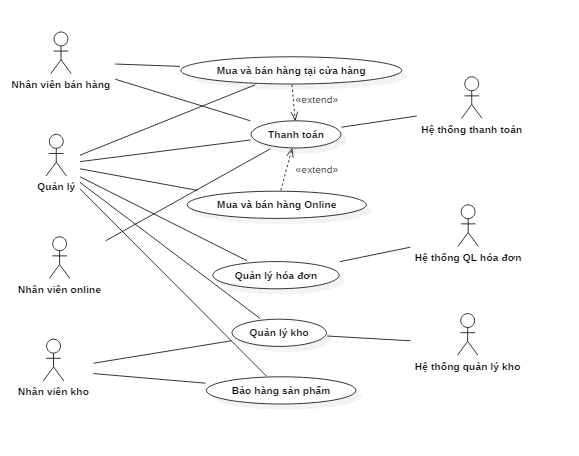
\includegraphics{3.png}
\end{figure}
\pagebreak

\fontsize{16}{20}\selectfont\section{Đặc tả chi tiết}
\fontsize{14}{20}\selectfont\subsection{Nghiệp vụ thanh toán}
Sau khi hoàn tất các bước chọn sản phẩm cũng như kiểm tra đầy đủ các thông tin cần thiết của khách hàng thông qua việc đặt hàng online hay đặt hàng trực tiếp, nhân viên thanh toán sẽ phải tạo một trang thanh toán trên hệ thống thanh toán hóa đơn của shop 

Trang thanh toán sẽ bao gồm những thông tin khách hàng đồng thời cũng cung cấp những chi tiết của đơn hàng bao gồm : 

\begin{itemize}
    \item Tên của hàng
    \item Bảng danh sách sản phẩm
    \item Tổng hóa đơn
    \item Khách thanh toán: Tiền mặt, Card. Thanh toán khi nhận hàng. chuyển khoảng
    \item Tiền thối
    \item Thông tin khách hàng: Họ Tên, Số điện thoại
    \item Ghi chú
    \item In hóa đơn
    \item Hoàn tất hóa đơn
\end{itemize}

Nhân viên thực hiện nhập thông tin sản phẩm thông qua barcode của sản phẩm, hệ thống sẽ dựa vào barde là tự động điền các thong tin của sản phẩm vào trang thanh toán

Trang thanh toán sẽ có nút Xóa cho từng sản phẩm trong trường hợp đã nhập sản phẩm vào trang thanh toán nhưng chưa thực hiện việc chốt hóa đơn mà khác muốn đổi hoặc không lấy sản phẩm đã được nhập trước đó 

Trường hợp khi mã sản phẩm không tồn tại trên hệ thống quản lý kho, hệ thống sẽ thông báo “ Sản phẩm không tồn tại” và không thực hiện nhập sản phẩm vào danh sách trên trang thanh toán.

Sau khi nhập thông tin sản phẩm ,trang thanh toán sẽ hiện nút “In bill” và cho phép nhân viên in bill cho khách kiểm tra và trang thanh toán sẽ cho phép nhập thông tin khách hàng. Nếu khách hàng là khách du lịch thì không cần lưu lại thông tin mà sẽ có một ID cố định cho khách du lịch là “KDL” 

Khi khách thanh toán nhân viên có thể chọn một hoặc nhiều phương thức gồm có 4 phương thức: tiền mặt. Thẻ. Chuyển khoản. Thanh toán khi nhận hàng ( dành cho đặt hàng online)  thanh toán, trang thanh toán sẽ hiện ra khung nhập số tiền cho phương thức thanh toán đó sau khi nhập đủ số tiền khách hàng phải thanh toán thì hệ thống sẽ hiện ra “ Done Bill” . 

Sau khi có đầy đủ thông tin khách hàng và số tiền phải thanh toán,  nhân viên phụ trách việc thanh toán sẽ nhấn “ Done bill “ hệ thống thanh toán sẽ  gửi thông điệp gồm thông tin hóa đơn đã thanh toán đến hệ thống quản lý hóa đơn để thực hiện việc tạo hóa đơn trên hệ thống quản lý hóa đơn và đến hệ thống quản lý hàng tồn để tự động cập nhật số lượng các sản phẩm đã được bán.Trang thanh toán thực hiệ in thêm một hóa đơn đã thanh toán. Hóa đơn đó sẽ không được thay đổi hay cập nhật nữa.Trang thanh toán đuộc đặt lại(reset)

Ngoài việc gửi thông tin đến hệ thống quản lý hóa đơn, Khi “ Done Bill”, hệ thống thanh toán đồng thời gửi thong tin đến hệ thống quản lý hàng tồn và hàng tồn tại cửa hàng sẽ tự động trừ đi các sản phẩm đã được thanh toán

Nếu hóa đơn được tạo nhưng không nhấn done thì hệ thống không gửi thông tin và không tạo hóa đơn trên hệ thống quản lý hóa đơn.
Khi hóa đơn được được tạo và đã có thông tin sản phẩm hoặc thông tin khách hàng, nhưng người dùng chọn nút thoát hoặc  đặt lại trang thanh toán. Hệ thống sẽ hiện thị cửa số với câu hỏi” Bạn muốn hủy hóa đơn” và 2 lựa chọn “ Không hủy hóa đơn” và “Hủy hóa đơn”. Khi người dùng chọn “Không hủy hóa đơn”, hệ thống sẽ tắt cửa sổ câu hỏi và vẫn giữ nguyên thông tin hiện đang có của hóa đơn.
\begin{figure}
    \centering
    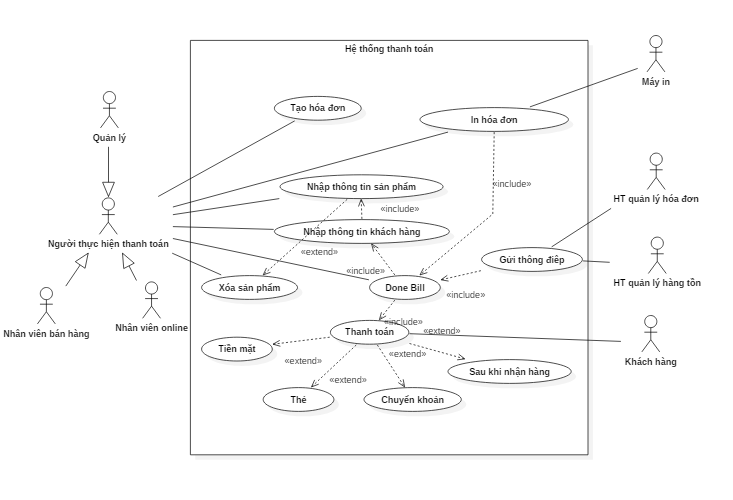
\includegraphics{4.png}
\end{figure}


\pagebreak

\begin{tabular}{|m{4cm}|m{12cm}|}
		\hline
		Use case name & Tạo hóa đơn\\
		\hline
		Scenario & Khách hàng muốn thanh toán sản phẩm\\
		\hline
		Triggering event & Sau khi khách hàng hoàn tất chọn mua sản phẩm và yêu cầu thanh toán\\
		\hline
		Brief description & Nhân viên mở trang thanh toán sản phẩm, tạo hóa đơn
Trang thanh toán hiển thị các mục thông tin cần được nhập của hóa đơn
Nhân viên nhập thông tin sản phẩm khách hàng muốn thanh toán thông qua Barcode sản phẩm, Thông tin khách hàng, Số tiền khách thanh toán.
Chốt hóa đơn, trang thanh toán gửi thông điêp thực hiện lưu hóa đơn và cập nhật số lượng sản phẩm có trong kho cửa hàng\\

		\hline
		 Actors & Nhân viên bán hàng, nhân viên online , quản lý\\
		 \hline
		 Related use case& \\
		 \hline
		 Stakeholders & \\
		 \hline
		 Precondition & Truy cập trang thanh toán trang thanh toán\\
		 \hline
		 Flow of event & 
		 	\begin{itemize}
		 		\item	Truy cập trang thanh toán
		 		\item 	Tạo hóa đơn
		 		\item	Trang thanh toán hiển thị các thông tin hóa đơn cần được nhập để thanh toán
		 		\item	Nhập thông tin sản phẩm
				\item In Hóa đơn chưa thanh toán
				\item	Nhập thông tin khách hàng
				\item	Khách hàng thanh toán
				\item	In hóa đơn đã thanh toán
				\item	Chốt hóa đơn ( Done bill)
				\item Gửi thông điệp đến hệ thống quản lý hàng tồn và hệ thống quản lý hóa đơn

		 	\end{itemize} \\
		 	\hline
		 	\end{tabular}
		 	
		 	\begin{tabular}{|m{4cm}|m{12cm}|}
		\hline
		Use case name & Xóa sản phẩm trên trang thanh toán  \\
		\hline
		Scenario & Khách hàng muốn đổi hoặc không lấy sản phẩm đó nữa \\
		\hline
		Triggering event & Đã nhập thông tin sản phẩm trên trang thanh toán nhưng chưa “ done bill” \\
		\hline
		Brief description & Nhân viên chọn sản phẩm khách hàng muốn bỏ khỏi hóa đơn thanh toán, chọn xóa sản phẩm \\
		\hline
		Actors & Nhân viên bán hàng, nhân viên online , quản lý \\
		\hline
		Related use case & Nhập thông tin sản phẩm\\
		\hline
		Stakeholders & \\
		\hline
		Precondition & Hóa đơn chưa được chốt (Done Bill) và sản phẩm đã được nhập trên trang thanh toán\\
		\hline
		
		Flow of event & 
			\begin{enumerate}
				\item Nhân viên chọn sản phẩm
				\item Chọn xóa sản phẩm
				\item Xóa sản phẩm khỏi hóa đơn
			\end{enumerate}\\
		\hline
		Exceptiom conditions & \\
		\hline
\end{tabular}\\[0.2cm]

\begin{tabular}{|m{4cm}|m{12cm}|}
		\hline
		Use case name & Thanh toán sản phẩm\\
		\hline
		Scenario & Khách hàng thanh toán sản phẩm\\
		\hline
		Triggering event & Chọn phương thức thanh toán cho hóa đơn\\
		\hline
		Brief description & Nhân viên chọn một hoặc nhiều phương thức thanh toán theo yêu cầu của khách hàng
Nhân viên nhập số tiền cho các phương thức thanh toán. Có thể chọn một hoặc nhiều phương thức  thanh toán theo yêu cầu của khách hàng. Gồm có 4 phương thức : Tiền mặt. Thẻ. Chuyển khoản, Thanh toán khi nhận hàng ( dành cho đặt hàng online).
\\
		\hline
		 Actors & Nhân viên bán hàng, nhân viên online , quản lý\\
		\hline
		Related use case & Done Bill\\
		\hline
		Stakeholders & \\
		\hline
		Precondition & Tạo trang thanh toán và nhập thông tin sản phẩm, nhập thông tin khác hàng, In bill chưa thanh toán\\
		\hline
		
		\end{tabular}
		
		\begin{tabular}{|m{4cm}|m{12cm}|}
		\hline
		Flow of event &
		\begin{enumerate}
				\item	Truy cập trang thanh toán
				\item Tạo hóa đơn
				\item Nhập thông tin sản phẩm
				\item In hóa đơn chưa thanh toán
				\item Nhập thông tin khách hàng
				\item \textbf{Chọn phương thức thanh toán}
				\item \textbf{Nhập số tiền cho phương thức thanh toán}
				\item In hóa đơn đã thanh toán
				\item Chốt hóa đơn (Done Bill)
				\item Gửi thông điệp đến hệ thống quản lý hàng tồn và hệ thống quản lý hóa đơn
			\end{enumerate}\\ 
		\hline
		Exceptiom conditions & \\
		\hline
\end{tabular}\\[0.3cm]

\begin{tabular}{|m{4cm}|m{12cm}|}
		\hline
		Use case name & Done bill\\
		\hline
		Scenario & Khách hàng thanh toán sản phẩm\\
		\hline
		Triggering event & Tạo trang thanh toán \\
		\hline
		Brief description & Brief description	Nhân viên thực hiện tạo hóa đơn thanh toán và đã nhập đủ các thông tin trên của hóa đơn, khi nhập đủ thông tin hóa đơn, trang thanh toán sẽ hiện nút “Done” 
Khi nhân viên thanh toán nhấn done bill, hệ thống thanh toán sẽ gửi thông điệp có thông tin hóa đơn đến hệ thống quản lý hóa đơn và hệ thống quản lý hàng tồn. Hóa đơn đó sẽ được chốt và không thể thay đổi trên trang thanh toán và máy in sẽ thực hiện in hóa đơn đã thanh toán. Trang thanh toán sẽ tự động refresh.\\
		\hline
		\end{tabular}
		\begin{tabular}{|m{4cm}|m{12cm}|}
        \hline
		 Actors & Nhân viên bán hàng, nhân viên online, quản lý\\
		\hline
		Related use case & Thanh toán, Nhập thông tin khách hàng, Gửi thông điệp, In hóa đơn đã thanh toán\\
		\hline
		Stakeholders & \\
		\hline
		Precondition & Nhân viên thực hiên tạo hóa đơn thanh toán và nhập thông tin hóa đơn và số tiền phải thanh toán\\
		\hline
		Flow of event & 
		\begin{enumerate}
			\item Truy cập trang thanh toán
			\item Tạo hóa đơn
			\item Nhập thông tin sản phẩm
			\item In Hóa đơn chưa thanh toán
			\item Nhập thông tin khách hàng
			\item Khách hàng thanh toán
			\item In hóa đơn đã thanh toán
			\item Chốt hóa đơn ( Done bill)
			\item Gửi thông điệp đến hệ thống quản lý hàng tồn và hệ thống quản lý hóa đơn
			\item Đặt lại trang thanh toán
        \end{enumerate}\\
	\hline
    Exceptiom conditions & \\
	\hline
\end{tabular}

\begin{tabular}{|m{4cm}|m{12cm}|}
		\hline
		Use case name & Gửi thông điệp\\
		\hline
		Scenario & Lưu thông tin hóa đơn và cập nhật hàng tồn kho\\
		\hline
		Triggering event & Nhân viên thanh toán chọn “Done Bill”\\
		\hline
		Brief description & Sau khi chốt hóa đơn, trang thanh toán sẽ gửi thông tin hóa đơn đến hệ thống quản lý hóa đơn để lưu lại hóa đơn trên CSDL, và gửi đến hệ thống quản lý kho hàng tồn để cập nhật hàng tồn tự dộng và lưu danh sách các sản phẩm đã được bán( xuất kho)\\
		\hline
		 Actors & Hệ thống quản lý kho, hệ thống quản lý hóa đơn,\\
		\hline
		Related use case & Done Bill\\
		\hline
		Stakeholders & \\
		\hline
		Precondition & Chốt hóa đơn\\
		\hline
		Flow of event & 
		\begin{enumerate}
			\item Nhân viên Done Bill
			\item Hiển thị cập nhật
			\item Hệ thống quản lý hóa đơn lưu lại thông tin hóa đơn
			\item Hệ thống quản lý hàng tồn tự động cập nhật trừ đi số lượng các món đã bán trong hóa đơn
		\end{enumerate}\\
	\hline
	Exceptiom conditions & Nếu trường hợp bị lỗi mạng hoặc lỗi hệ thống không gửi thông điệp được, Trang thanh toán hiển thị thông báo “ Cập nhật không thanh công”, Trang thanh toán vẫn giữ nguyên \\
	\hline
\end{tabular}
\pagebreak
\fontsize{14}{20}\selectfont\subsection{Quy trình quản lý hóa đơn}
Hệ thống quản lý hóa đơn cung cấp dịch vụ cho đối tượng : Người quản lý 

Hệ thống quản lý hóa đơn chỉ được truy cập và điều hàng bởi người quản lý cửa hàng. Ví dụ như: Tạo hóa đơn, thay đổi , chỉnh sủa thông tin khách hàng ,cập nhật thông tin và truy xuất thông tin, xem thông tin, thêm xóa thông tin, hóa đơn,..

Hệ thống hóa đơn chỉ được quản lý bởi người quản lý chủ cửa hàng  vì lí do bảo vệ thông tin khách hàng (Họ Tên, Số điện thoại khách hàng ) đảm bảo rằng không có bất kì ai có thể truy cập hoặc đánh cắp thông tin khách hàng dùng cho một số mục đích khác. 

Những thông tin gồm có trên một hóa đơn được quản lý bởi hệ thống bao gồm:
    \begin{itemize}
        \item Tên cửa hàng (Chi nhánh Nguyễn Trãi, TPHCM; chi nhánh Hà Nội)
        \item Thời gian
        \item ID Khách hàng (Số điện thoại khách hàng)
        \item Danh sách các sản phẩm
        \item Số tiền thanh toán(Tiền mặt, Thanh toán khi nhận hàng, Chuyển khoản)
    \end{itemize}
Những thông tin hóa đơn có thể được truy xuất, tìm kiếm theo: Tên cửa hàng, Ngày giờ, Id khách hàng, mã sản phẩm, tên sản phẩm, size sản phẩm. Khi người quản lý cần tìm hóa đơn sẽ dựa theo những thông tin trên để truy xuất dữ liệu từ hệ cơ sở dữ liệu giúp việc tìm kiếm trở nên nhanh chóng và thuận tiện. 

Sau khi qua quy trình thanh toán và tạo hóa đơn do nhân viên cửa hàng thực hiện trên trang thanh toán sản phẩm của cửa hàng. 
Mỗi khi nhân viên nhấn nút  “Done bill  “trên trang thanh toán Hệ thống sẽ tạo một hóa đơn dựa vào những thông tin cần thiết ở trên nếu chưa có thông tin hóa đơn đó trên hệ thống. Mỗi hóa đơn sẽ có được cấp một mã hóa đơn riêng. Và thêm vào danh sách hóa đơn trên hệ thống và hệ cơ sở dũ liệu. 

Khi một hóa đơn đã được chốt trên trang thanh toán, đã được “ Done” thì hóa đơn đó không thể được thay đổi trên trang thanh toán. Nhưng hóa đơn có thể được quản lý thay đổi hoặc cập nhật thông tin cho hóa đơn.
Quản lý có thể thay đổi thông tin của hóa đơn trên hệ thống. Sẽ có 2 ngữ cảnh khi thay đổi thông tin hóa đơn trên hệ thống. :
    \begin{itemize}
         \item Thay đổi thông tín sản phẩm(số lượng, phần trăm,ghi chú): Thêm hoặc xóa sản phẩm trong đơn hàng, chỉnh sửa phần trăm giảm giá hoặc ghi chú của từng sản phẩm
         \item Thay đổi thông tin khách hagf: thay đôi tên hoặc ID khách hàng
    \end{itemize}
Sau khi hoàn tất việc thay đổi thông tin, Quản lý sẽ chốt hóa đơn, Nếu thông tin số lượng sản phẩm của các hóa đơn được thay đổi, hệ thống quản lý hóa đơn sẽ gửi một thông điệp thông báo đến hệ thống quản lý hàng tồn cập nhật lại các số lượng các sản phẩm xuất kho cửa hàng (đã bán). Khi thông điệp được gửi thành công, hệ thống sẽ hiển thị thông báo “Đã cập nhật” 
Nếu thông tin được thay đổi là thông tin khách hàng, hệ thống sẽ sửa đổi thông tin khác hàng theo thông tin quản lý đã cập nhật và hiện thị thông báo “đã cập nhật”

-Nếu sau khi đã thay đổi thông tin hóa đơn nhưng không ấn chốt hóa đơn (Done) nhưng đã thoát trang hoặc trang hóa đơn được đặt lại (refresh)  thì hệ thống sẽ hiện thông báo “ Bạn có muốn cập nhật hóa đơn không?” với 2 nút “Có” và “ Không”
Nếu người dùng chọn” Có” Hệ thống thực hiện cập nhật lại hóa đơn và hệ thống hiển thị thông báo “Đã cập nhật” . Nếu không hệ thống hủy thông tin cập nhật và không thay đổi hóa đơn.

Khi quản lý xóa một hóa đơn trên hệ thống quản lý hóa đơn, hệ thống quản lý hóa đơn sẽ gửi một thông điệp gồm thông tin và số lượng các sản phẩm trong hóa đơn đó đến hệ thống quản lý hàng tồn , hệ thống quản lý hàng tồn sẽ tự động cập nhật  nhập kho số lượng các món trong hóa đơn vào hàng tồn của cửa hàng. Và thông báo với người quản lý hóa đơn đã được xóa.

Quản lý có thể in danh sách các món đã bản được theo thời gian được xác định (Ví dụ: từ ngày 26/8/2019 đến 8/9/2019) từ  danh sách này nhân viên kho sẽ dựa trên các món sản phẩm đã được bán để nhập các món sản phẩm này từ kho tổng về lại kho cửa hàng.
    \begin{figure}
        \centering
        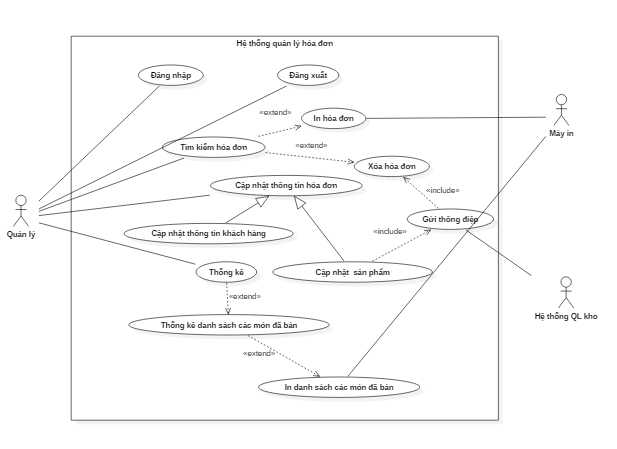
\includegraphics{5.png}
    \end{figure}

\begin{tabular}{|m{4cm}|m{12cm}|}
		\hline
		Use case name & Cập nhật hóa đơn\\
		\hline
		Scenario & Hóa đơn được thanh toán trên hệ thống thanh toán \\
		\hline
		Triggering event & Thông tin hóa đơn thiếu hoặc sai. \\
		\hline
		Brief description & Thay đổi thông tin của hóa đơn đã có trên hệ thống quản lý hóa đơn. Có 2 ngữ cảnh thay đổi thông tin hóa đơn: 
-	Thay đổi thông tin của các sản phẩm trong hóa đơn ( thêm, xóa ). Khi thay đổi số lượng hoặc sản phẩm trong hóa đơn hệ thống sẽ gửi một thông điệp đến hệ thống quản lý kho. Hệ thống quản lý kho sẽ cập nhật hàng tồn của kho
-	Thay đổi thông tin khách hàng: Thay đổi khi thông tin khách hàng bị sai hoặc thiếu\\
		\hline
		 Actors &  Actors	Quản lý, Hệ thống quản lý kho\\
		\hline
		Related use case & In bill/ Done bill, Đăng nhập\\
		\hline
		Stakeholders & Server lưu trữ\\
		\hline
	\end{tabular}
    
    \begin{tabular}{|m{4cm}|m{12cm}|}
        \hline
		Precondition & Hóa đơn đã được tạo trên hệ thống\\
		\hline
		Flow of event & 
			\begin{enumerate}
				\item Quản lý đăng nhập hệ thống 
				\item Tim kiếm hóa đơn cần cập nhật 
				\item Chọn phương thức cập nhật 
				\item Cập nhật thông tin hóa đơn
				\item Done
				\item Hiện thông báo
				\item Hệ thống gửi thông điệp đế hệ thống quản lý kho
 
			\end{enumerate}\\
		\hline
		Exceptiom conditions & Nếu sau khi đã thay đổi thông tin hóa đơn nhưng không ấn chốt hóa đơn (Done) nhưng đã thoát trang hoặc trang hóa đơn được đặt lại (refresh)  thì hệ thống sẽ hiện thông báo “ Bạn có muốn cập nhật hóa đơn không?” với 2 nút “Có” và “ Không”
		
Nếu người dùng chọn” Có” Hệ thống thực hiện cập nhật”. Nếu không hệ thống hủy thông tin cập nhật và không thay đổi hóa đơn 
 \\
		\hline
    \end{tabular}
	
\begin{tabular}{|m{4cm}|m{12cm}|}
		\hline
		Use case name & Tìm kiếm hóa đơn\\
		\hline
		Scenario & Cần truy xuất thông tin hóa đơn\\
		\hline
		Triggering event & Quản lý thực hiện truy xuất hóa đơn\\
		\hline
		Brief description & Quản lý tìm kiếm và truy xuất hóa đơn dựa trên một hoặc nhiều phương thức thông  qua các thông tin sau: 
		\begin{itemize}
			\item ID khách hàng
			\item Tên sản phẩm
			\item Ngày tạo hóa đơn
			\item Cửa hàng ( chi nhánh )
			\item Theo ngày 
		\end{itemize}				
		Sau khi chọn các phương thức truy xuất hóa đơn, hệ thống sẽ hiển thị danh sách các hóa đơn nằm theo thông tin được tìm kiếm. Danh sách có thể có không hoặc nhiều hóa đơn\\
		\hline
		 Actors & Người quản lý\\
		\hline
		Related use case & Đăng nhập, In hóa đơn, Xóa hóa đơn\\
		\hline
		Stakeholders & Server luu trữ hóa đơn\\
		\hline
		Precondition & Hệ thống có tồn tại hóa đơn\\
		\hline
		Flow of event & 
			\begin{enumerate}
				\item Quản lý đăng nhập hệ thống
				\item Chọn mục tìm kiếm hóa đơn
				\item Nhập thông tin hóa đơn cần tìm kiếm
				\item Hệ thống hiển thị danh sách các hóa đơn
			\end{enumerate}\\
		\hline
		Exceptiom conditions & \\
		\hline
\end{tabular}		
	
\begin{tabular}{|m{4cm}|m{12cm}|}
		\hline
		Use case name & Xóa hóa đơn\\
		\hline
		Scenario & Khách hủy đơn hàng hoặc đơn hàng bị trùng \\
		\hline
		Triggering event & Quản lý thực hiện việc xóa hóa đơn\\
		\hline
		Brief description & Brief description	Quản lý xóa đăng nhập hệ thống và tìm kiếm hóa đơn cần được xóa. Quản lý chọn hóa đơn và chọn “Xóa hóa đơn”.
		 
Sau khi hóa đơn được xóa, hệ thống hiển thị thông báo “ Hóa đơn đã được xóa” và gửi một thông điệp đến hệ thống quản lý kho đế cập nhật (cộng thêm) số lượng các sản phẩm trong kho.

Đặt lại trang quản lý hóa đơn ( refresh trang )
\\
		\hline
		 Actors &  Người quản lý\\
		\hline
		Related use case & Đăng nhập, Tìm kiếm hóa đơn\\
		\hline
		Stakeholders & Server luu trữ hóa đơn \\
		\hline
		Precondition & Hóa đơn đã được tạo trên hệ thống \\
		\hline
		Flow of event & 
			\begin{enumerate}
				\item Quản lý đăng nhập hệ thống 
				\item Tìm kiếm hóa đơn
				\item Chọn hóa đơn
				\item Chọn xóa hóa đơn
				\item Gửi thông điệp đến hệ thống quản lý kho
				\item Hệ thống hiển thị thông báo
				\item Refresh trang 
			\end{enumerate}\\
		\hline
		Exceptiom conditions & Khi xóa hóa đơn nhưng nếu thông điệp gửi không thành công đến hệ thống quản lý kho, hệ thống sẽ hiển thì thông báo “Lỗi không thể cập nhật”. Các thao tác xóa hóa đơn sẽ bị hủy và đặt lại trang thanh toán.\\
		\hline
\end{tabular}

		\begin{tabular}{|m{4cm}|m{12cm}|}
		\hline
		Use case name & Thống kê danh sách các sản phẩm đã bán\\
		\hline
		Scenario & Cần danh sách các sản phẩm đã bán để nhập kho CH các món đã được bán theo ngày \\
		\hline
		Triggering event & \\
		\hline
		Brief description & Hệ thống sẽ thống kê các sản phẩm đã bán được thông qua dữ liệu của danh sách xuất kho cửa hàng. Quản lý có thể chọn thống kê các sản phẩm đã bán theo các thông tin sau:
		\begin{itemize}
			\item Từ ngày .. Đến ngày…
			\item Mã sản phẩm
			\item Tên sản phẩm
		\end{itemize}\\
		\hline
		 Actors & Người quản lý\\
		\hline
		Related use case & Đăng nhập hệ thống, thống kê\\
		\hline
		Stakeholders & Server luu trữ hóa đơn danh sách xuất kho cửa hàng\\
		\hline
		Precondition & Có tồn tại danh sách xuất kho CH\\
		\hline
		Flow of event & 
			\begin{enumerate}
				\item Quản lý đăng nhập hệ thống 
				\item Chọn thống kê
				\item Chọn mục thống kê danh sách sản phẩm đã bán
				\item Chọn phương thức thống kê
				\item Hệ thống hiển thị danh sách

			\end{enumerate}\\
		\hline
		Exceptiom conditions & -Khi mã sản phẩm hoặc tên sản phẩm người dùng muốn thống kê không tồn tại, Hệ thống hiển thị thông báo “ sản phẩm không tồn tại”
		
- Khi thống kê theo ngày, Nếu người dùng nhập ngày trong “Từ ngày” lớn hơn ngày của “Đến ngày”. Hệ thống thông báo” Nhập sai thời gian”\\
		\hline
\end{tabular}

\fontsize{14}{20}\selectfont\subsection{Quy trình quản lí kho}
\fontsize{13}{20}\selectfont
Nhân viên kho và quản lý là 2 tác nhân tác động lên hệ thống quản lý kho. Để quản lý kho hàng tồn hệ thống sẽ tập trung vào việc xuất, nhập kho của các sản phẩm và thông qua việc đối chiếu các danh sách nhập, xuất để đảm bảo tính xác thực và tin cậy của kho. 
Trang quản lý kho sẽ có những chức năng chính: Tìm kiếm, kiểm tra sản phẩm trong kho, Tạo danh sách nhập kho, xuất kho

\fontsize{14}{20}\selectfont\textbf{Tìm kiếm, kiểm tra sản phẩm }

Khi nhân viên truy cập trang quản lý kho, nhân viên chọn kho cần tìm kiếm. Hệ thống sẽ hiển thị danh sách các sản phẩm trong kho. Nhiên viên có thể tìm kiếm,lọc danh sách sản phẩm dựa trên các thông tin theo các thông tin:
    \begin{itemize}
        \item Mã sản phẩm
        \item Tên sản phẩm
        \item Size
        \item Loại
        \item Giá sản phẩm
        \item Số lượng
    \end{itemize}
Hệ thống sẽ trả về danh sách sản phẩm với các thông tin được tìm kiếm \\

\fontsize{14}{20}\selectfont\textbf{Tạo dánh sách xuất kho}
Nhân viên kho sẽ thực hiện tạo danh sách xuất kho khi muốn xuất sản phẩm đó về một kho khác.

Sau khi tạo danh sách, nhân viên kho sẽ thực hiện nhập thông tin sản phẩm thông qua  Mã Sản phẩm, Trang quản lý sẽ tự động điền những thông tin của sản phẩm dựa trên mã sản phẩm và thêm vào bảng danh sách các sản phẩm xuất kho 

Danh sách sẽ hiển thị những thông tin gồm: 
    
    \begin{itemize}
        \item Ngày nhập kho
        \item Kho xuất đi
        \item Danh sách sản phẩm xuất kho
        \item Tổng số sản phẩm
    \end{itemize}
Sau khi nhập đầy đủ các sản phẩm và thông tin sản phẩm nhập kho, nhân viên kho sẽ thực hiện chốt danh sách ( Done) . Trang quản lý sẽ gửi thông điệp cập nhật cơ sở dữ liệu  trừ đi số lượng các sản phẩm được xuất kho trong danh sách các sản phẩm trong kho.\\

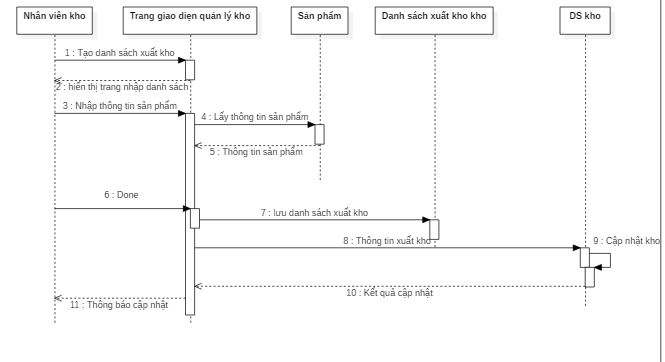
\includegraphics[scale = 0.5]{20.png}



\fontsize{14}{20}\selectfont\textbf{Tạo danh sách nhập kho}
Nhập kho sẽ gồm có 3 ngữ cảnh: Nhập kho các sản phẩm từ kho tổng về kho cửa hàng hoặc từ cửa hàng về cửa hàng và Nhập kho các sản phẩm từ hãng về kho tổng, Khách hàng đổi trả sản phẩm
 
Sau khi tạo danh sách, nhân viên kho sẽ thực hiện nhập thông tin sản phẩm thông qua Mã sản phẩm , 

Danh sách sẽ hiển thị những thông tin gồm: 

\begin{enumerate}
        \item Ngày xuất kho
        \item Kho Xuất đi
        \item Mã sản phẩm
        \item Category:
            \begin{itemize}
                \item Giày dép
                \item Quần áo
                \item Phụ kiện
            \end{itemize}
        \item Size
        \item Số lượng
        \item Tổng sản phẩm
\end{enumerate}
Các sản phẩm khi được nhập vào danh sách có thể được xóa bởi nhân viên kho để phòng trường hợp nhập sai hoặc dư trong lúc nhập các sản phẩm vào danh sách.
Sau khi nhập đầy đủ các sản phẩm và thông tin sản phẩm trong danh sách nhân viên sẽ thực hiện chốt danh sách và danh sách khôn g thể bị thay đổi. 

\begin{enumerate}
    \item 	Nếu ngữ cảnh (1), nhân viên sẽ chọn mục “ nhập từ hãng về” và  mục ghi chú của danh sách nhập kho là “Danh sách sản phẩm được nhập từ hãng về ngày ../ .. /  .. “ 
    \item 	Nếu ngữ cảnh (2), nhân viên sẽ chọn mục “ Nhập từ kho khác”, và thực hiện nhập mã danh sách xuất kho muốn đối chiếu. trang quản lý sẽ gửi thông điệp yêu cầu đối chiếu danh sách nhập kho vói danh sách xuất kho với mã tương ứng với mã danh sách xuất kho được nhập vào. Mục ghi chú của danh sách nhập kho sẽ có nội dung “  Danh sách sản phẩm được nhập từ kho .. (Mã danh sách xuất kho) ngày ../  ../  .. “.
    \item 	Nếu ngữ cảnh (3), nhân viên sẽ chọn mục “ Khách đổi trả”, Mục ghi chú của danh sách nhập kho sẽ là “ Khách đổi trả ngày ../ ../ ..”
\end{enumerate}

Sau khi nhập đủ các sản phẩm được nhập, nhân viên sẽ chốt danh sách nhập kho.
\begin{itemize}
    \item Ngữ cảnh (2), nếu danh sách nhập kho khớp với danh sách xuất kho tương ứng, trang quản lý kho sẽ gửi thông điệp thực hiện lưu danh sách nhập kho và cập nhật cộng thêm số lượng sản phẩm trong kho được nhập về theo danh sách các sản phẩm nhập kho, thông báo nhập kho thành công và trở về trang chủ quản lý kho. Ngược lại, Trang quản lý sẽ thông báo số lượng sản phẩm bị sai lệch giữa hai danh sách, hiển thi yêu cầu kiểm tra lại danh sách. 
    \item Ngữ cảnh (1) và (3), Trang quản lý kho sẽ thực hiện lưu danh sách nhập kho và cập nhật số lượng sản phẩm được nhập kho theo danh sách.
\end{itemize}
Khi danh sách được tạo có thông tin sản phẩm, nếu người dùng thoát danh sách. Hệ thống sẽ hiện thị của số với nội dung “ Danh sách đang có sản phẩm. Bạn có muốn thoát” với 2 lựa chọn” Có” và “ Không”. Nếu người dùng chọn  “có”, hệ thống sẽ hủy danh sách đượcc tạo và thoát trở về trang chủ. Ngược lại, Hệ thống sẽ tắt cửa sổ thông báo và giữ nguyên trang danh sách

Nếu danh sách không có sản phẩm, sau khi nhấn “done” Hệ thống sẽ hiển thị thông báo “danh sách không có sản phẩm” và không thực hiện tạo danh sách và cập nhật hàng tồn.

\fontsize{14}{20}\selectfont\textbf{Tạo sản phẩm}
Khi sản phẩm mới được nhập về thì sẽ chưa có dữ liệu trong hệ thống nên ta  sẽ thực hiện việc tạo dữ liệu cho sản phẩm thông qua mã barcode mà hãng đã cung cấp.

Khi tạo sản phẩm mới, từ dữ liệu barcode mà hãng đã cung cấp ta lấy được tên sản phẩm, size, Mã SP, màu sắc giá của sản phẩm sẽ do quản lý quy định và được nhập bởi quản lý hoặc nhân viên quản lý kho. 

Sau khi đã điền đầy đủ các thông tin sản phẩm, nhân viên kho hoặc quản lý sẽ hoàn tất việc tạo dữ liệu cho sản phẩm mới. , Nhân viên nhấn “Tạo”. Nếu đã có thông tin sản phẩm trên cơ sở dữ liệu, hệ thống sẽ báo lỗi “Sản phẩm đã tồn tại”.Nếu không có,

Hệ thống sẽ tự động thêm dữ liệu vào bảng CSDL của các kho với số lượng sản phẩm mặc định là 0.

Nếu người dùng nhập thiếu thông tin nhưng đã ấn tạo, Hệ thống sẽ hiển thị thông báo yêu cầu nhập đủ thông tin và đánh dấu đỏ các thông tin chưa được nhập. \\
    \begin{figure}
        \centering
        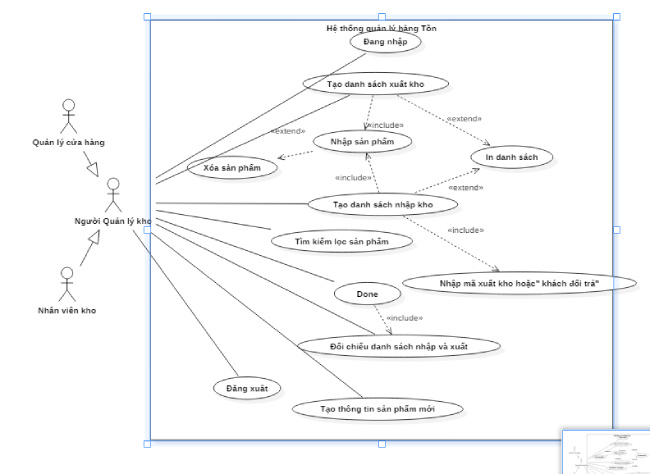
\includegraphics{6.png}
    \end{figure}


\begin{tabular}{|m{4cm}|m{12cm}|}
		\hline
		Use case name & Tạo danh sách xuất kho \\
		\hline
		Scenario & Xuất kho sản phẩm \\
		\hline
		Triggering event & Khi sản phẩm được xuất khỏi kho \\
		\hline
		Brief description & Nhân viên kho sẽ thực hiện tạo danh sách xuất kho. Nhập thông tin sản phẩm,Chọn kho xuất đi, Chốt danh sách. Trang quản lý kho gửi thông điệp đến hệ cơ sở dữ liệu để cập nhật sô lượng sản phẩm của các sản phẩm được xuất đi \\
		\hline
		 Actors & Nhân viên kiểm kho, quản lý cửa hàng..\\
		\hline
		Related use case &  \\
		\hline
		Stakeholders & \\
		\hline
		Precondition &\\
		\hline
		Flow of event & \begin{enumerate}
		    \item	Truy cập trang quản lý kho
        	\item Tạo danh sách xuất kho
            \item Chọn kho xuất đi 
            \item Nhập thông tin sản phẩm
            \item Chốt danh sách ( Done bill)
	       \item Gửi thông điệp đến hệ thống quản lý hàng tồn và hệ thống quản lý hóa đơn
	    \end{enumerate}  \\
		\hline
		Exceptiom conditions &	Khi danh sách được tạo có thông tin sản phẩm, nếu người dùng thoát danh sách. Hệ thống sẽ hiện thị của số với nội dung “ Danh sách đang có sản phẩm. Bạn có muốn thoát” với 2 lựa chọn” Có” và “ Không”. Nếu người dùng chọn  “có”, hệ thống sẽ hủy danh sách đượcc tạo và thoát trở về trang chủ. Ngược lại, Hệ thống sẽ tắt cửa sổ thông báo và giữ nguyên trang danh sách \\
		\hline
\end{tabular}

\begin{tabular}{|m{4cm}|m{12cm}|}
		\hline
		Use case name & Tạo danh sách nhập kho \\
		\hline
		Scenario & Sản phẩm được nhập kho \\
		\hline
		Triggering event & \begin{enumerate}
		    \item Sản phẩm từ kho khác về
        	\item Khách hàng đổi trả sản phẩm
            \item Sản phẩm từ nhà phân phối nhập về

	    \end{enumerate}\\
		\hline
		Brief description & Nhân viên kho sẽ thực hiện tạo danh sách nhập kho, nhập thông tin các sản phẩm được nhập vào danh sách, Chọn kho nhập về, Chọn ngữ cảnh nhập kho:
		
		\begin{enumerate}
		    \item Nhập kho các sản phẩm từ kho khác:  Nhập mã danh sách xuất kho muốn đối chiếu.
        	\item Nhập kho sản phẩm khách đổi trả: Chọn mục khách đổi trả
            \item Nhập kho các sản phẩm từ hãng nhập về: Chọn mục “ Nhập từ hãng “
        \end{enumerate}
        Nhân viên chốt danh sách. Nếu có mã danh sách xuất kho, Trang quản lý kho sẽ gửi yêu cầu đối chiếu với danh sách xuất kho có mã danh sách xuất kho tương ứng với mã được nhập vào.
        Gửi thông điêp đến Cơ sở dữ liệu để cập nhật số lượng sản phẩm. \\

		\hline
		 Actors & Nhân viên kiểm kho, quản lý cửa hàng..\\
		\hline
		Related use case &  \\
		\hline
		Stakeholders & \\
		\hline
		Precondition &\\
		\hline
	\end{tabular}
    
    \begin{tabular}{|m{4cm}|m{12cm}|}
    \hline
		Flow of event & \begin{enumerate}
		    \item	Truy cập trang quản lý kho
        	\item Tạo danh sách xuất kho
            \item Chọn kho xuất đi 
            \item Nhập thông tin sản phẩm
            \item Chốt danh sách ( Done bill)
	       \item Gửi thông điệp đến hệ thống quản lý hàng tồn và hệ thống quản lý hóa đơn
	    \end{enumerate}  \\
	
		\hline
		Exceptiom conditions &	\begin{enumerate}
                \item Ngữ cảnh khi nhập kho các sản phẩm từ kho khác về, nếu số lượng sản phẩm không khớp với số lượng sản phẩm trong danh sách xuất kho được đối chiếu, trang thanh toán sẽ thông báo số lượng sản phẩm không khớp và không cho phép nhập kho 
                \item Khi danh sách được tạo có thông tin sản phẩm, nếu người dùng thoát danh sách. Hệ thống sẽ hiện thị của số với nội dung “ Danh sách đang có sản phẩm. Bạn có muốn thoát” với 2 lựa chọn” Có” và “ Không”. Nếu người dùng chọn  “có”, hệ thống sẽ hủy danh sách đượcc tạo và thoát trở về trang chủ. Ngược lại, Hệ thống sẽ tắt cửa sổ thông báo và giữ nguyên trang danh sách
        \end{enumerate}\\
		\hline
\end{tabular}

	\begin{tabular}{|m{4cm}|m{12cm}|}
		\hline
		Use case name & Tìm kiếm , kiểm tra sản phẩm \\
		\hline
		Scenario & Tìm kiếm sản phẩm trong hàng tồn của kho \\
		\hline
		Triggering event & \\
		\hline
		Brief description & Nhân viên kho đăng nhập vào hệ thống quản lý kho, chọn kho cần tìm kiếm sản phẩm và có thể lọc sản phẩm trên dữ liệu kho CH hoặc kho tổng theo một hoặc nhiều thông tin sau:
		\begin{itemize}
			\item Mã sản phẩm
			\item Tên sản phẩm
			\item Size
			\item Loại 
			\item Giá sản phẩm
		\end{itemize}
		Hệ thống sẽ xuất ra danh sách các sản phẩm theo các thông tin trên.\\
		\hline
		 Actors & Nhân viên kiểm kho, quản lý cửa hàng.\\
		\hline
		Related use case & Đăng nhập, Đăng xuất \\
		\hline
		Stakeholders & \\
		\hline
		Precondition & Tạo danh sách nhập và xuất kho\\
		\hline
		Flow of event & 
			\begin{enumerate}
			\item Đăng nhập hệ thống
			\item Chọn kho
			\item Chọn thông tin cần tìm kiếm
			\item Hệ thống hiển thị danh sách sản phẩm 
			\end{enumerate}\\
		\hline
		Exceptiom conditions & Nếu không có sản phẩm tìm kiếm, Hệ thống sẽ trả về danh sách trống \\
		\hline
	\end{tabular}

\begin{tabular}{|m{4cm}|m{12cm}|}
		\hline
		Use case name & Tạo sản phẩm mới  \\
		\hline
		Scenario & Tạo thông tin cho sản phẩm mới\\
		\hline
		Triggering event & Khi có sản phẩm mới được nhập về\\
		\hline
		Brief description & Nhân viên kho đăng nhập vào hệ thống quản lý kho, chọn mục tạo sản phẩm mới. Nhân viên sẽ lần lượt nhâp các thông tin sau:
		\begin{itemize}
			\item Barcode
			\item Mã sản phẩm
			\item Tên sản phẩm 
			\item Màu sản phẩm
			\item Loại sản phẩm
			\item Size
			\item Giá tiền
		\end{itemize}
		Sau khi nhập đầy đủ các thông tin trên, Nhân viên nhấn “Tạo”. Nếu đã có thông tin sản phẩm trên cơ sở dữ liệu, hệ thống sẽ báo lỗi “Sản phẩm đã tồn tại”.Nếu không có,
hệ thống sẽ tạo thông tin sản phẩm mới trong cơ sở dữ liệu của các kho và mặc định số lượng sản phẩm sẽ là 0.\\
		\hline
		 Actors & Nhân viên kiểm kho, quản lý cửa hàng.\\
		\hline
		Related use case & Đăng nhập, Đăng xuất \\
		\hline
		Stakeholders & \\
		\hline
		Precondition & Đăng nhập hệ thống, Sản phẩm chưa tồn tại trên hệ thống \\
		\hline
		Flow of event & 
			\begin{enumerate}
				\item Đăng nhập hệ thống 
				\item Chọn mục tạo sản phẩm mới
				\item Nhập thông tin sản phẩm
				\item Nhấn phím Tạo
				\item Hiển thị thông báo
			\end{enumerate}\\
		\hline
    \end{tabular}
    
    \begin{tabular}{|m{4cm}|m{12cm}|}
        \hline
        Exceptiom conditions & \begin{enumerate}
            \item Nếu sản phẩm đã tồn tại trên CSDL, hệ thống sẽ thông báo “ sản phẩm đã tồn tại”.
		    \item	Nếu người dùng nhập thiếu thông tin nhưng đã ấn tạo, Hệ thống sẽ hiển thị thông báo yêu cầu nhập đủ thông tin và đánh dấu đỏ các thông tin chưa được nhập
        \end{enumerate}	\\
		\hline
	\end{tabular}
\pagebreak

\fontsize{14}{20}\selectfont\textbf{Biểu đồ lớp cho hệ thống quản lý hóa đơn\\}
\fontsize{13}{20}\selectfont

Một khách hàng khi mua sản phẩm sẽ được lưu lại gồm có điện thoại, Tên khách. 
Cửa hàng sẽ gồm có các thông tin là Mã Cửa hàng, Tên Cửa hàng 
Hóa đơn của khách bao gồm Mã hóa đơn ( do hệ thống cấp cho một hóa đơn ), Mã khách hàng, Mã cửa hàng, Ngày 
Mỗi sản phẩn sẽ gồm có  Mã sản phẩm  Tên sản phẩm, Size,Loại sản phẩm, Giá tiền, 
Trong một hóa đơn sẽ có một hoặc nhiều sản phẩm, Một sản phẩm có thể thuộc một hoặc nhiều hóa đơn.Mỗi sản phẩm thuộc hóa đơn sẽ được cấp cho Mã hóa đơn của hóa đơn đó, 

Kho gồm có 3 kho đó là : Kho tổng, Kho cửa hàng SG, Kho cửa hàng HN. 
Một kho sẽ gồm các thành phần : Mã kho, Tên Kho, Tổng số lượng 
Một kho gồm có một hoặc nhiều sản phẩm, và sản phẩm có thể thuộc một hoặc nhiều kho và gồm có số lượng của từng sản phẩm trong kho

Khi một sản phẩm được bán ở cửa hàng thì sẽ được lưu vào danh sách các sản phẩm đã bán,Nhân viên kho sẽ nhập các sản phẩm từ kho tổng về lại kho cửa hàng dựa trên danh sách các sản phẩm đã bán sẽ xuất ra được danh sách các sản phẩm sẽ được nhập kho. 

Dựa trên danh sách các sản phẩm sẽ được nhập kho thì nhân viên kho sẽ tạo danh sách các sản phẩm xuất kho từ kho tổng . Danh sách xuất kho gồm các thành phần sau: Mã xuất kho, Mã kho ( Mã kho xuất đi ), Ngày xuất, Tổng số lượng xuất. Một danh sách xuất kho gồm một hoặc nhiều sản phẩm và mỗi sản phẩm sẽ thuộc một hoặc nhiều danh sách xuất kho. Mỗi sản phẩm xuất kho sẽ có : Mã xuất kho, Mã sản phẩm, Size, Barcode, Tên sản phẩm,  Một kho sẽ có một hoặc nhiều danh sách xuất kho. 

Danh sách nhập kho sẽ dựa trên danh sách sản phẩm xuất kho sẽ gồm có: Mã nhập kho, Mã kho (kho được nhập), Ngày nhập kho, Tổng số lượng nhập. Một danh sách sẽ có một hoặc nhiều sản phẩm. Mỗi sản phẩm sẽ có: Mã nhập kho, Mã sản phẩm, Size, Barcode, Tên sản phẩm, Size, .  Một kho sẽ có một hoặc nhiều danh sách nhập kho.\\

\begin{figure}
    \centering
    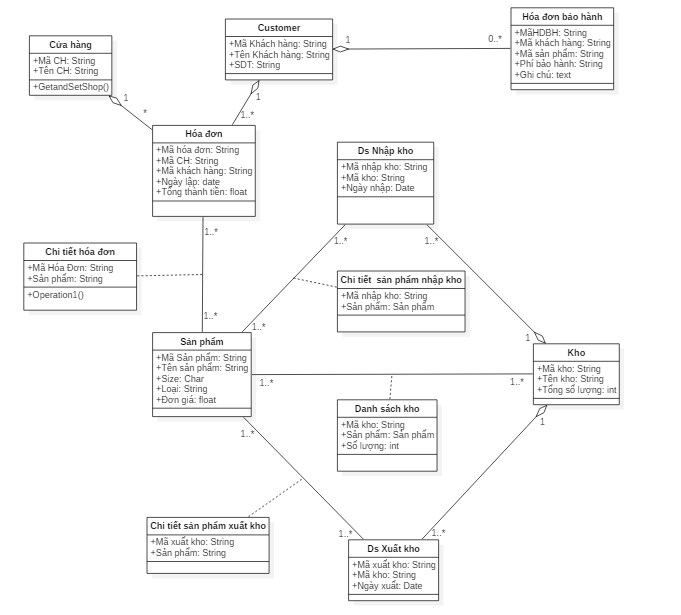
\includegraphics{7.png}
    \caption{Biểu đồ Class}
\end{figure}

\begin{figure}
    \centering
    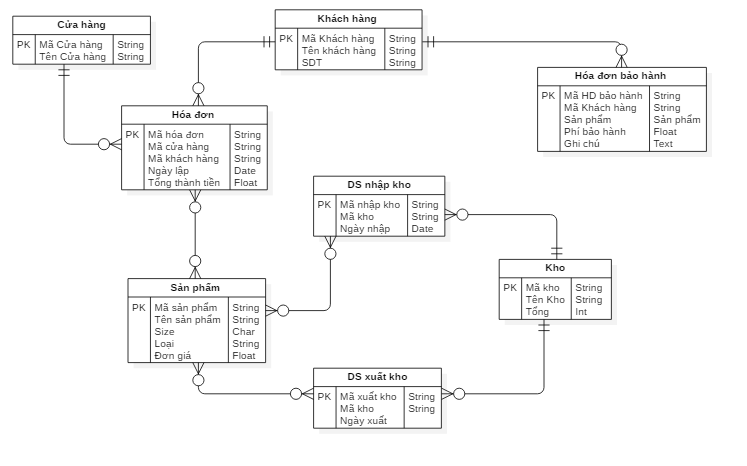
\includegraphics{16.png}
    \caption{Biểu đồ ERD}
\end{figure}
\pagebreak
\fontsize{14}{20}\selectfont\textbf{Biểu đồ tuần tự hệ thống thanh toán và quản lí hóa đơn\\}
\fontsize{13}{20}\selectfont
Nhân viên thực hiện mở trang thanh toán lên và nhập thông tin trên trang thanh toán Nhân viên có thể nhập barcode sản phẩm của sản phầm trang thanh toán sẽ gửi mã barcode hoặc thông tin nhập đến hệ cơ sở dư liệu lưu trư thông tin sản phẩm. Hệ cơ sở dữ liệu sẽ truy xuất và gửi thông tin sản phẩm gồm tên sản phẩm, giá sản phẩm ngược lại cho trang thanh toán. Nhân viên thực hiện nhập lần lượt các sản phẩm khách hàng đã chọn. Trang thanh toán sẽ trả về tổng số tiền phải thanh toán Nhân viên nhập số tiền khách thanh toán cho hóa đơn,thông tin khách hàng Sau khi đã thanh toán ,  nhân viên sẽ chốt hóa đơn -done bill- trang thanh toán sẽ tạo form in bill gửi thôg tin hoá đơn đến printer để thực hiện việc in hoá đơn. Trang thanh toán cũng đồng thời gửi thông tin đến hệ thống quản lý hoá đơn, hệ thống sẽ tạo một hoá đơn trên hệ cơ sở dữ liệu gồm các thông tin của hoá đơn và thêm thông tin các sản phẩm đã được bán. Trang thanh toán sẽ yêu cầu nhập thông tin khách hàng. 

Sau khi trang quản lý hóa đơn nhận dữ liệu, trang thanh toán sẽ gửi dữ liệu đến hệ thống quản lý hàng tồn. Hệ thống quản lý hàng tồn sẽ tự động cập nhật và trừ đi số lượng các sản phẩm đã bán.\\
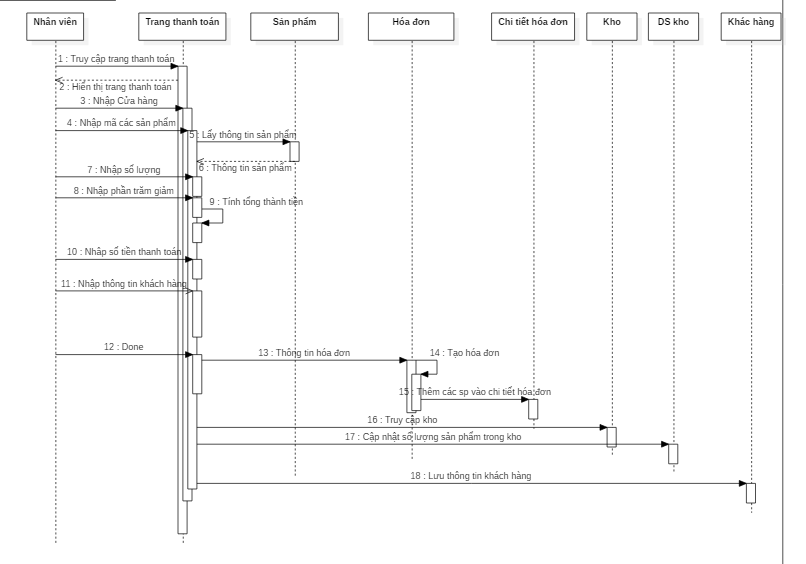
\includegraphics[scale = 0.8]{8.png}

\pagebreak
\fontsize{14}{20}\selectfont\textbf{Cập nhật hóa đơn}

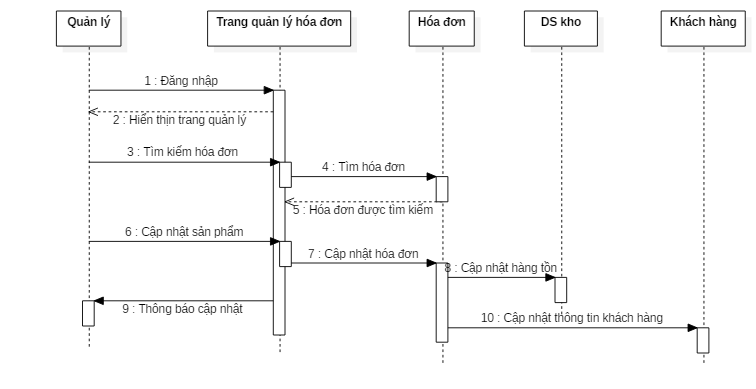
\includegraphics[scale = 0.8]{10.png}

\pagebreak

\pagebreak
\fontsize{14}{20}\selectfont\subsection{Biểu đồ tuần tự và hoạt động cho quản lý kho}
  \fontsize{14}{20}\selectfont\textbf{Xuất kho}

\centering
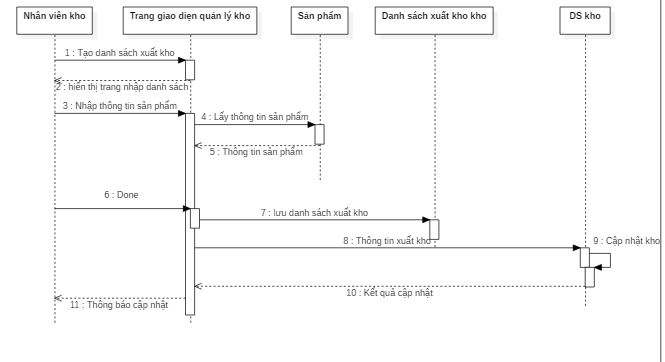
\includegraphics[scale=0.8]{20.png}\\
\fontsize{13}{20}\selectfont\caption{Biểu đồ Squence}\\


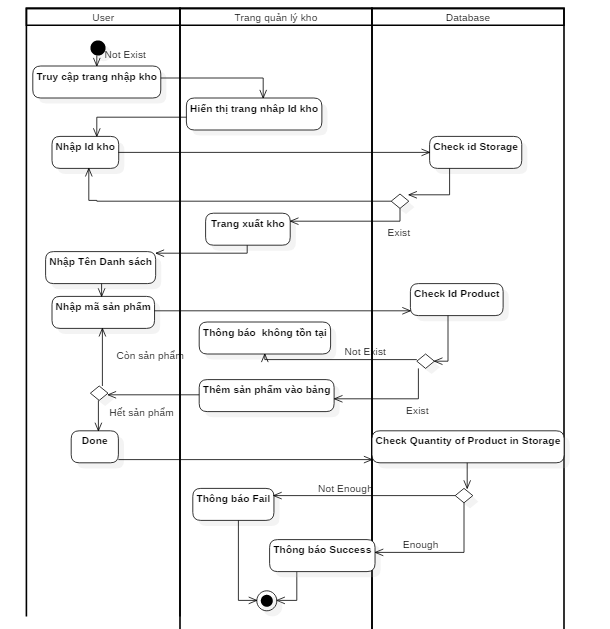
\includegraphics[scale = 0.7]{32.png}\\
\fontsize{13}{20}\selectfont\caption{Biểu đồ Acitvity}\\


\pagebreak
\centering






\pagebreak

\fontsize{14}{20}\selectfont\textbf{Nhập kho các sản phẩm được xuất từ kho khác về}

\fontsize{13}{20}\selectfont

Nhân viên kho sẽ tạo một bảng nhập kho, mỗi danh sách nhập kho sẽ có mã nhập kho riêng dựa trên ngày nhập kho ( vd : Nhập kho ngày 25/8/2019, mã nhập kho sẽ có dạng NK250819) và nhậ thông tin sản phẩm thông qua barcode các sản phẩm vào bảng nhập kho . Nhân viên thực hiện nhập thông tin của danh sách nhập kho gồm :Tên danh sách nhập kho, thông tin các sản phẩm nhận kho, và chọn ngữ cảnh nhập kho.
Nếu nhân viên chọn ngữ cảnh nhập kho các sản phẩm được xuất từ kho khác về thì, nhân viên sẽ thực hiện nhập thêm mã xuất kho của danh sách xuất kho muốn đối chiếu
	
Nhân viên khi thực hiện việc “ done”  hệ thống sẽ đối chiếu danh sách nhập kho với danh sách xuất kho có mã xuất kho tương ứng được nhập vào. 
Nếu danh sách đủ các số lượng sản phẩm trong danh sách xuất kho sẽ thực hiện việc tạo và lưu danh sách nhập kho ,cập nhật hàng tồn kho dựa trên số lượng sản phẩm được nhập thêm trong danh sách và hiển thị thông báo cho người dùng

%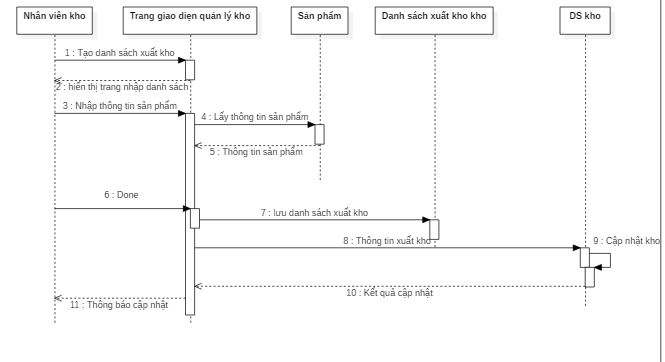
\includegraphics[scale = 0.8]{20.png}

\begin{center}
  \fontsize{14}{20}\selectfont\textbf{Biểu đồ Squence}
    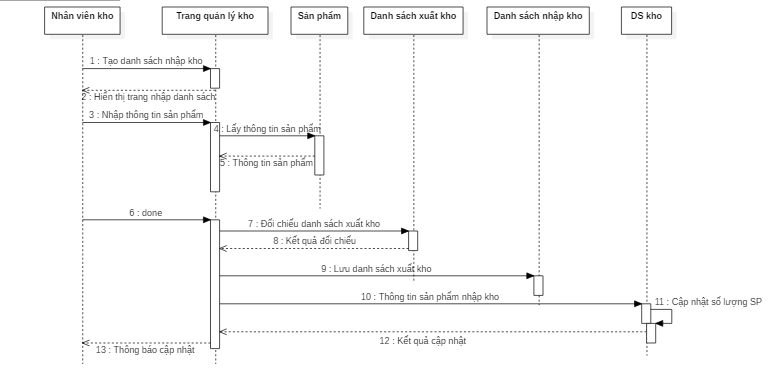
\includegraphics[scale=0.8]{11.png}  \\
    \caption{Biểu đồ Squence}
\end{center}

\pagebreak
\centering
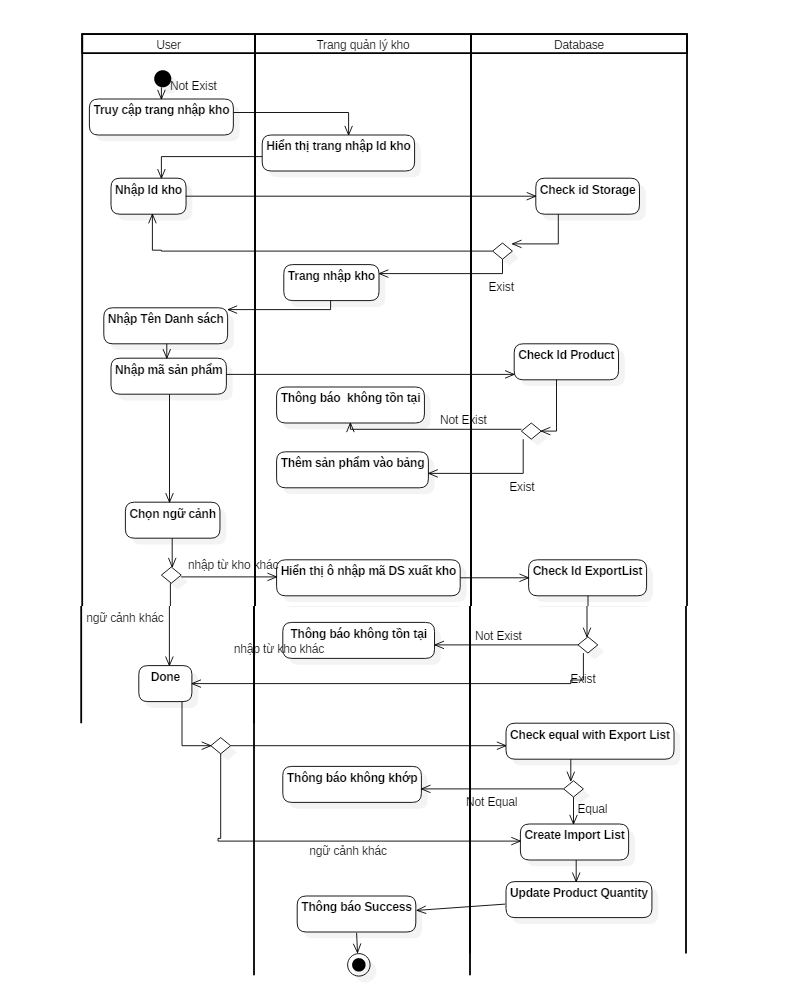
\includegraphics[scale = 0.5]{35.png}\\
\fontsize{13}{20}\selectfont\caption{Biểu đồ Activity}


\pagebreak

\pagebreak
\centering
\fontsize{14}{20}\selectfont\textbf{Tạo sản phẩm mới}\\


\fontsize{13}{20}\selectfont

Khi sản phẩm mới được nhập về thì sẽ chưa có dữ liệu trong hệ thống nên ta  sẽ thực hiện việc tạo dữ liệu cho sản phẩm thông qua mã barcode mà hãng đã cung cấp.
Khi tạo sản phẩm mới, từ dữ liệu barcode mà hãng đã cung cấp ta lấy được tên sản phẩm, size, Mã SP, màu sắc giá của sản phẩm sẽ do quản lý quy định và được nhập bởi quản lý hoặc nhân viên quản lý kho. 
Sau khi đã điền đầy đủ các thông tin sản phẩm, nhân viên kho hoặc quản lý sẽ hoàn tất việc tạo dữ liệu cho sản phẩm mới. Hệ thống sẽ thêm dữ liệu sản phẩm vừa được tạo vào bảng Product .

Việc nhập kho sẽ diên ra như nhập kho các sản phẩm đã có dữ liệu trước đó, hệ thống sẽ tự động cập nhật số lượng sản phẩm đã được nhập kho 

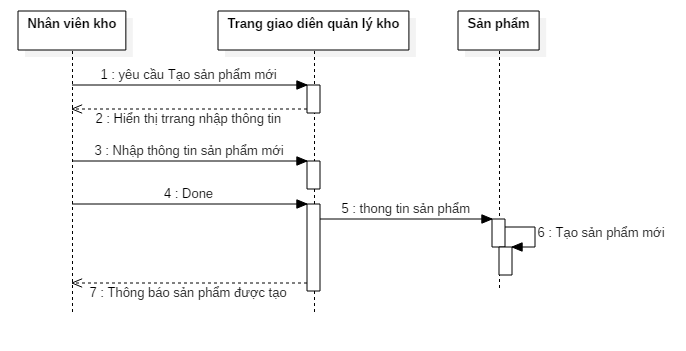
\includegraphics[scale = 0.8]{12.png}

\pagebreak

\fontsize{16}{20}\selectfont\section{Demo Project}
Đồ án được thực hiện dựa trên framework Django. Để thực thi được project, cần cài đặt hai môi trường
\begin{itemize}
    \item Python 3
    \item Django
\end{itemize}
\fontsize{14}{20}\selectfont\subsection{Cài đặt môi trường Python}

\fontsize{13}{20}\selectfont

Vì framework Django được lập trình bằng ngôn ngữ Python, vậy nên chúng ta cần phải cài đặt môi trường Python cho thiết bị

Step 1: Truy cập trang web http:\\python.org (Trang chủ Python) sau đó click vào thẻ Download 

        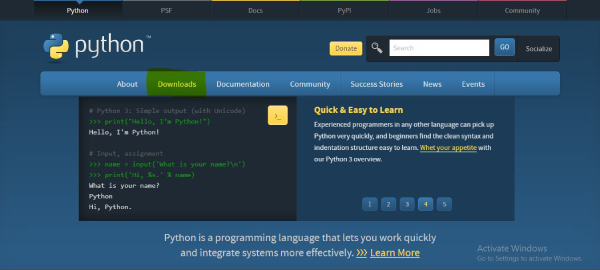
\includegraphics{5.jpg}
\pagebreak

Step 2: Click vào khung Download Python như trên hình

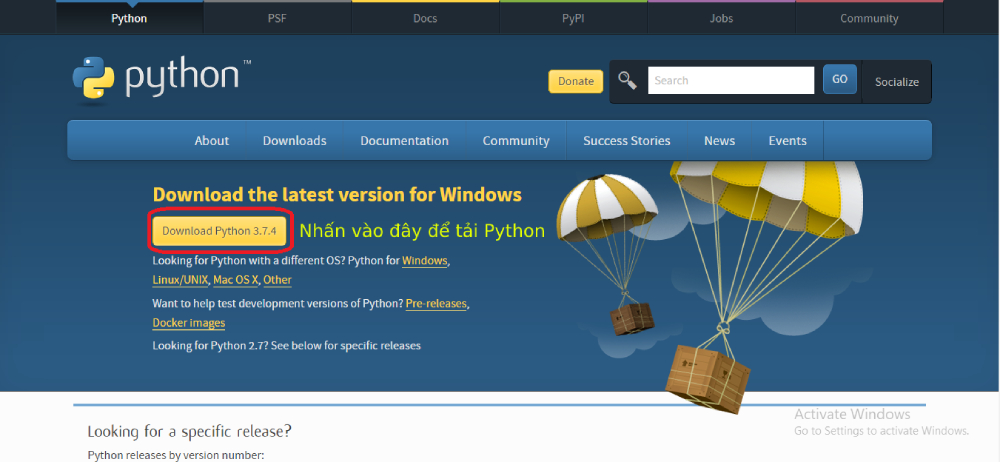
\includegraphics[sacle=0.4]{6.jpg}
	
Step 3: Chờ để tải file Python

Step 4: Sau kho tải xong, mở file vừa tải , xuất hiện bảng như sau,click check vào ô Add Python 3.7 to Path để cài đặt môi trường ngôn ngữ Python không cần phải dùng cách thủ công và nhấn Install Now

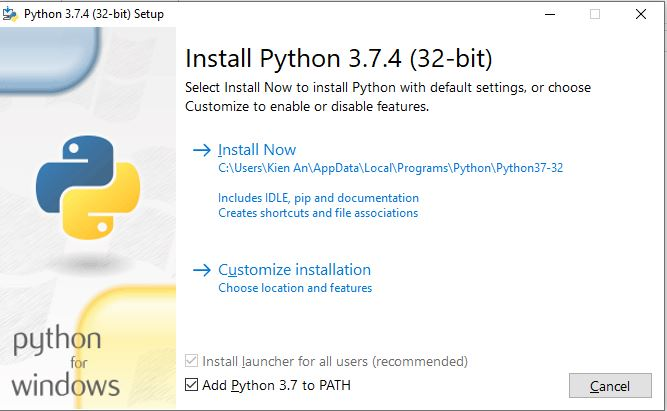
\includegraphics{7.jpg}

Step 5: Chờ khoảng 3 - 4 phút để cài đặt môi trường Python

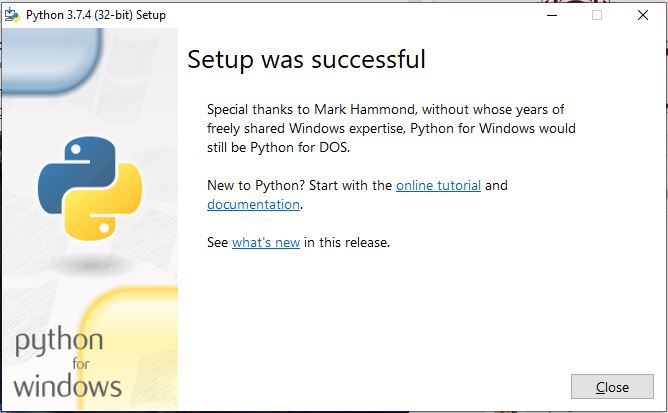
\includegraphics[scale =1]{8.jpg}

Xuất hiện ra bảng này là đã cái đặt thành công!!!

\fontsize{14}{20}\selectfont\subsection{Cài đặt Framework Django}

\fontsize{13}{20}\selectfont

Sau khi cài đặt thành công ngôn ngữ Python, chúng ta tiền hành cài đặt framework Django
Step 1: Mở cửa số Command Prompt (CMD) bằng cách nhấn tổ hợp phím Window + R và nhấn cmd hoặc có thể mở bằng tìm cmd trên công cụ search của Win 10.

    \begin{figure}[htp]
        \centering
        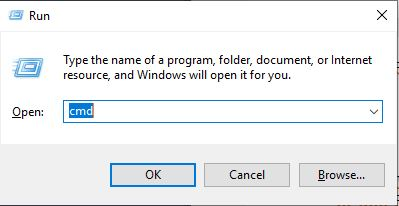
\includegraphics{9.jpg}
        \caption{Mở bằng lệnh Run}
    \end{figure}
    
\begin{figure}[htp]
        \centering
        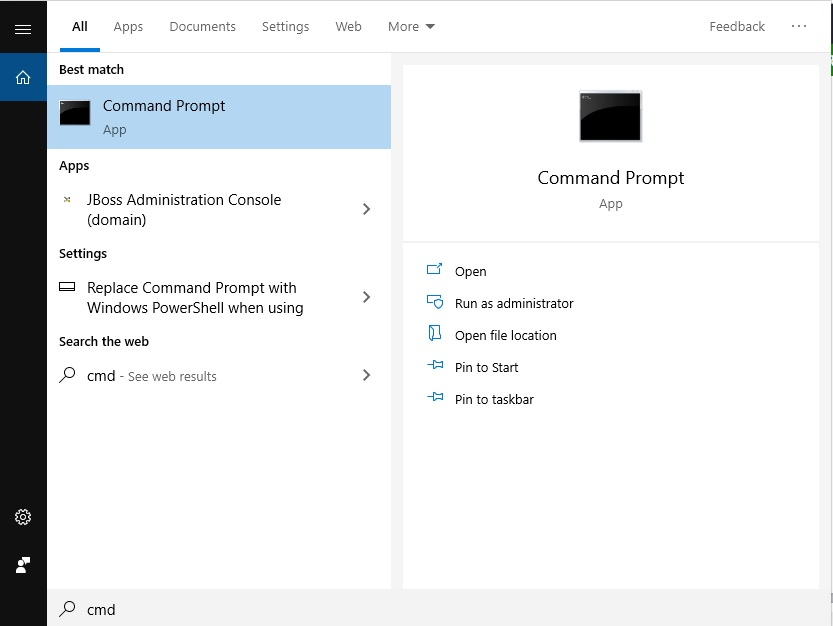
\includegraphics[scale=0.5]{10.jpg}
        \caption{mở bằng cách tìm trên thanh công cụ search}
    \end{figure}

\pagebreak

Step 2: Hiển thị danh sách các phiên bản của django thì ta gõ lệnh 
pip search django trên cửa số cmd mà chúng ta đã mở ra

    \begin{figure}[htp]
        \centering
        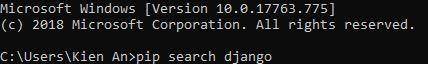
\includegraphics{11.jpg}
        \caption{Lệnh tìm kiếm phiên bản của Django}
    \end{figure}
    
     \begin{figure}[htp]
        \centering
        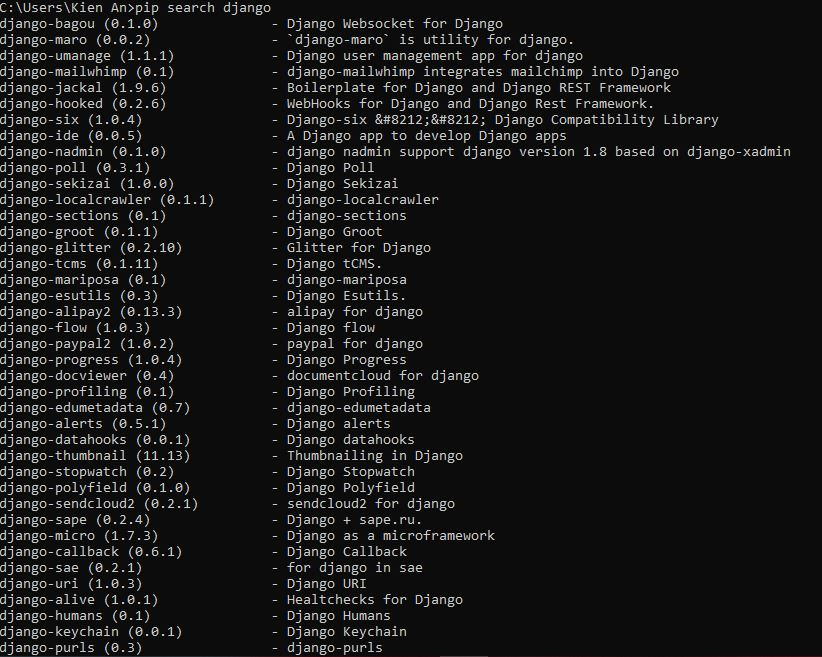
\includegraphics[scale=0.5]{12.jpg}
        \caption{một số phiên bản đầu tiên của Django}
    \end{figure}

Cài đặt Django ta dùng câu lệnh \textbf{pip install django} để cài đặt phiên ban mới nhất của Django hoặc \textbf{pip install django 2.0.6} để cài đặtđúng phiên bản 2.0.6 của Django

     \begin{figure}[htp]
        \centering
        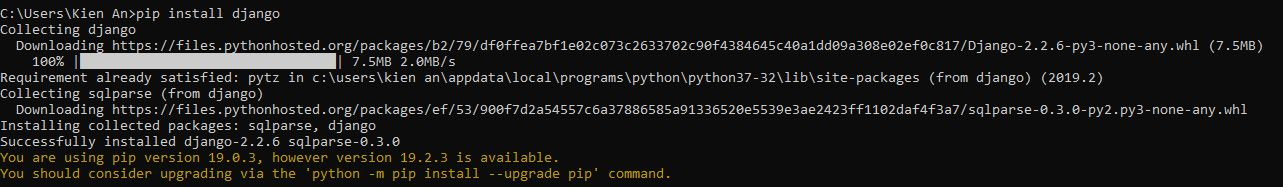
\includegraphics[scale=0.5]{13.jpg}
        \caption{câu lệnh tải và thông báo cài đặt hoàn thành}
    \end{figure}

Cách cài đặt Django chính là dùng folder source của chính framework này
	
Dẫn tệp tin code vào folder và thực hiện lệnh như hình bên dưới sẽ cài đặt đc framework Django

\fontsize{14}{20}\selectfont\textbf{Chạy Project}

\fontsize{13}{20}\selectfont

Sau khi cài đặt pythonthực hiện lệnh, mở command line : pip install- r requirements.txt  

Sau khi hoàn tất việc download, gõ lệnh : python manage.py runserver

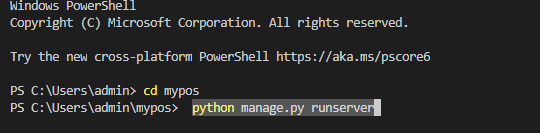
\includegraphics[scale = 0.6]{13.png} \\

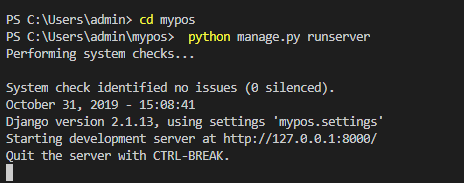
\includegraphics[scale = 0.6]{14.png}\\

Ta nhấp vào đường dẫn mà cmd cung cấp. Sẽ xuất hiện ra trang web của Project\\

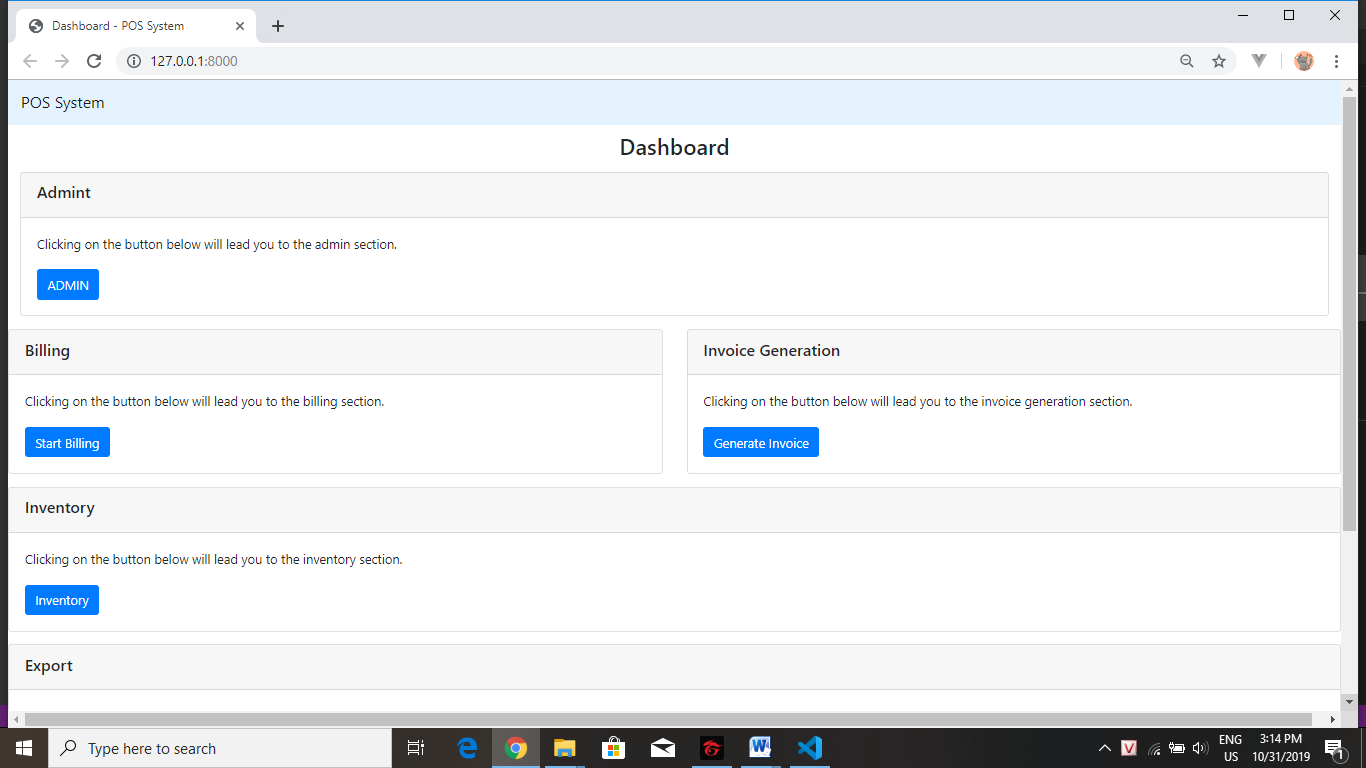
\includegraphics[scale = 0.4]{15.png}

\pagebreak
\begin{itemize}
    \item Đăng nhâp trang admin
    \item User: admin
    \item Password:123456
\end{itemize}




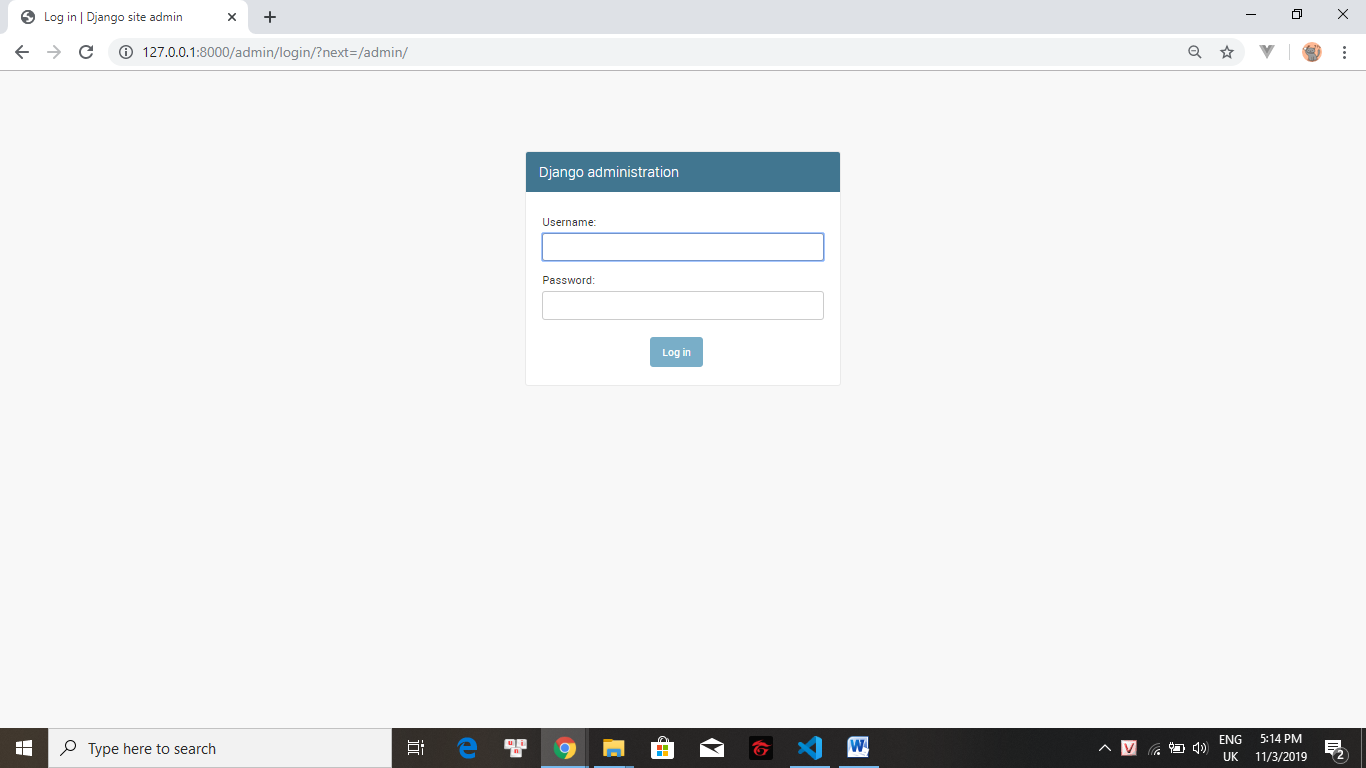
\includegraphics[scale = 0.4]{21.png}

Trang thanh toán\\

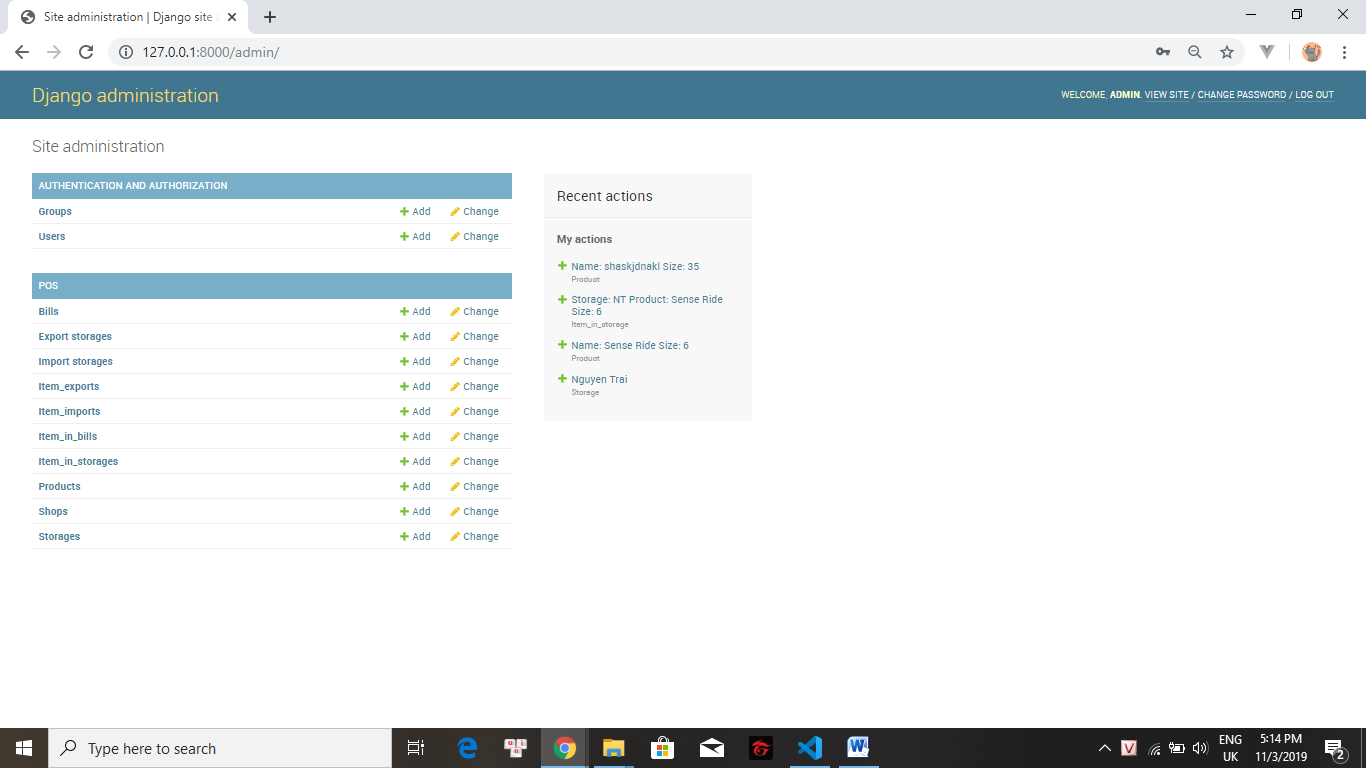
\includegraphics[scale = 0.4]{22.png}

\pagebreak


Bước 1: Chọn Billing\\

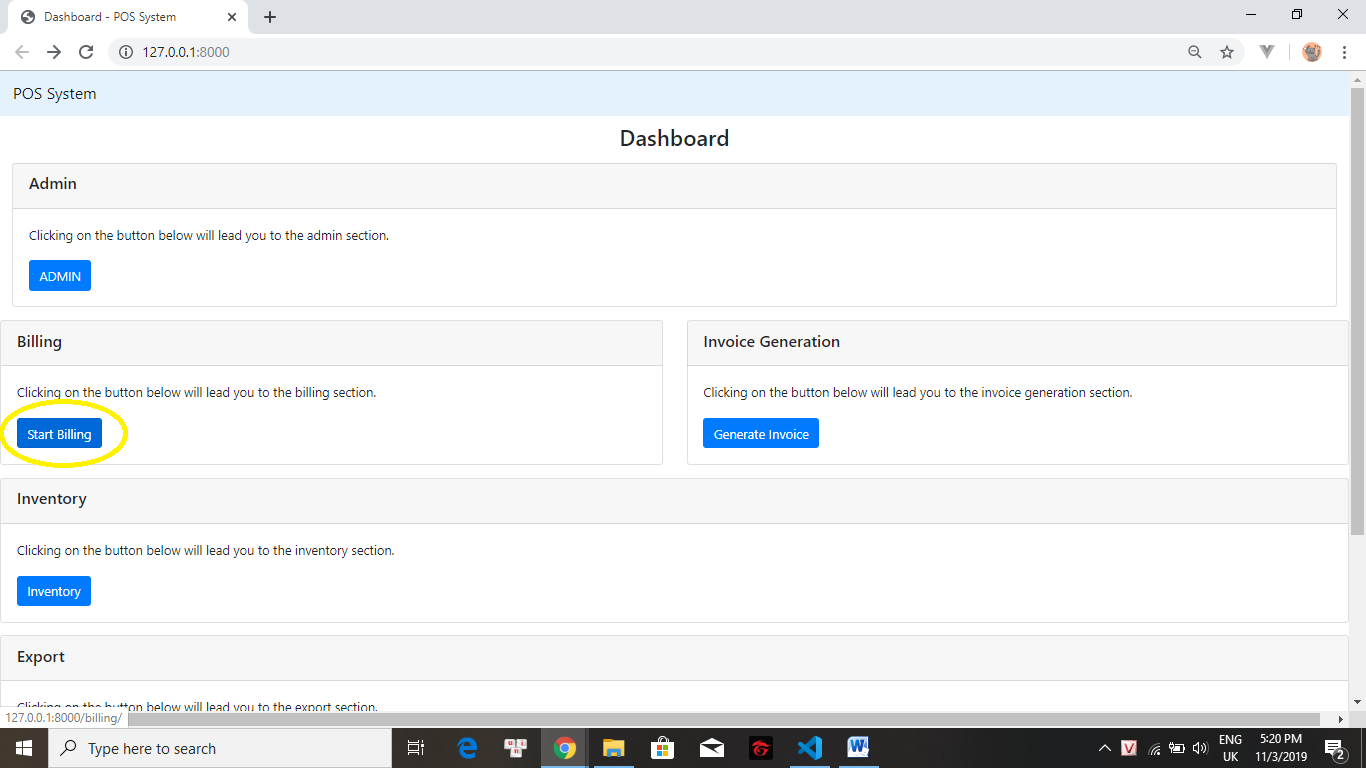
\includegraphics[scale = 0.4]{23.png}

Bước 2: Nhập ID Kho, Go

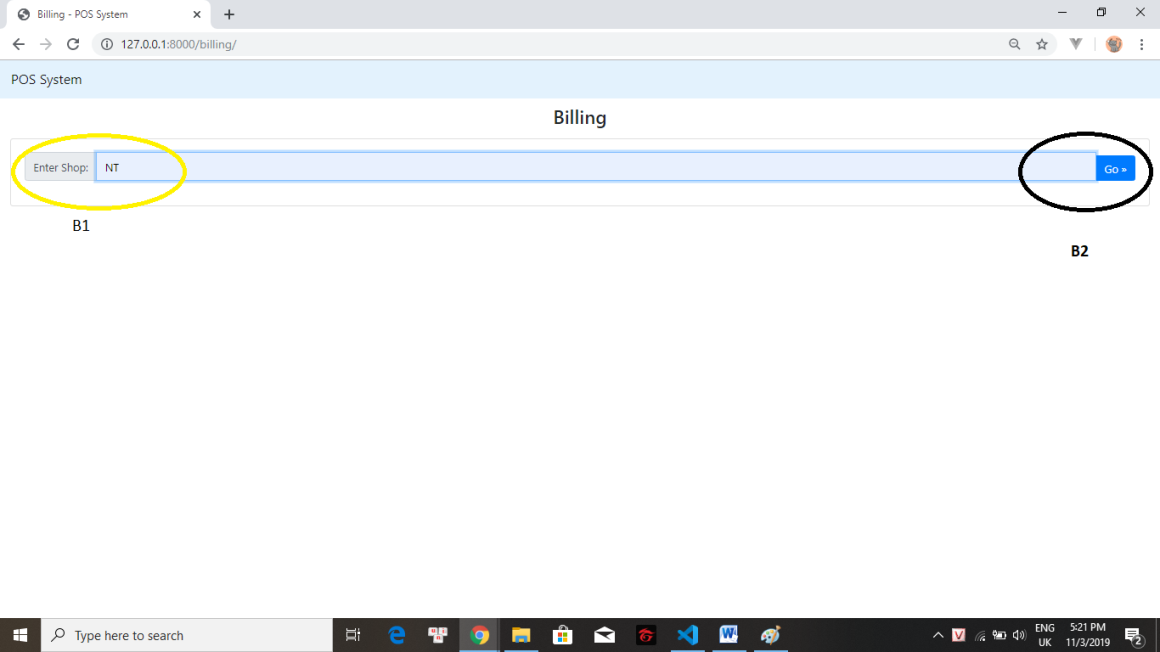
\includegraphics[scale = 1]{24.png}

\pagebreak

Bước 3: Nhập ID sản phẩm trong ô Enter Id Prodcut, GO \\

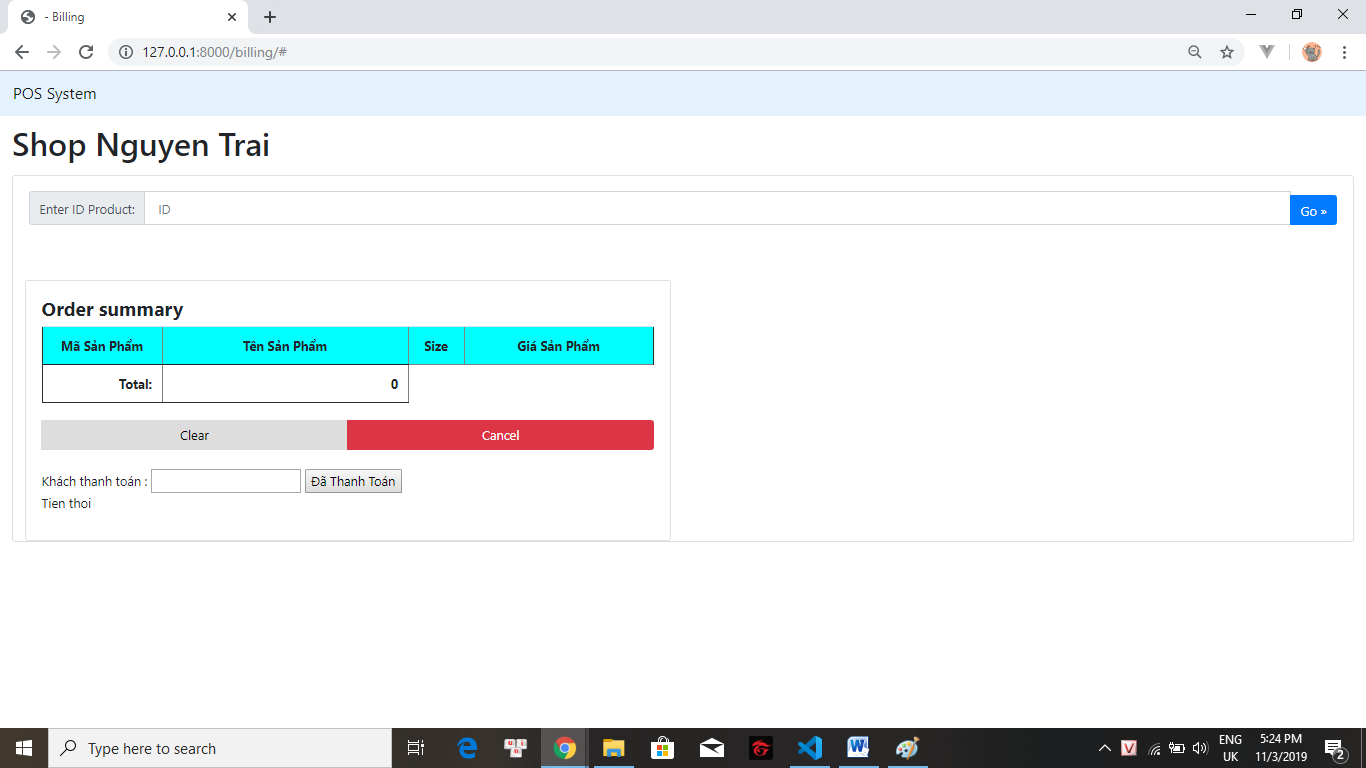
\includegraphics[scale=0.5]{25.png}

Bước 4: Nhập số tiền khách thanh toán, Chọn Đã Thanh Toán. Nếu số tiền khách thanh toán lớn hơn hoặc bằng thì trang thanh toán sẽ hiển thị tiền thối và nút “ Bill” \\

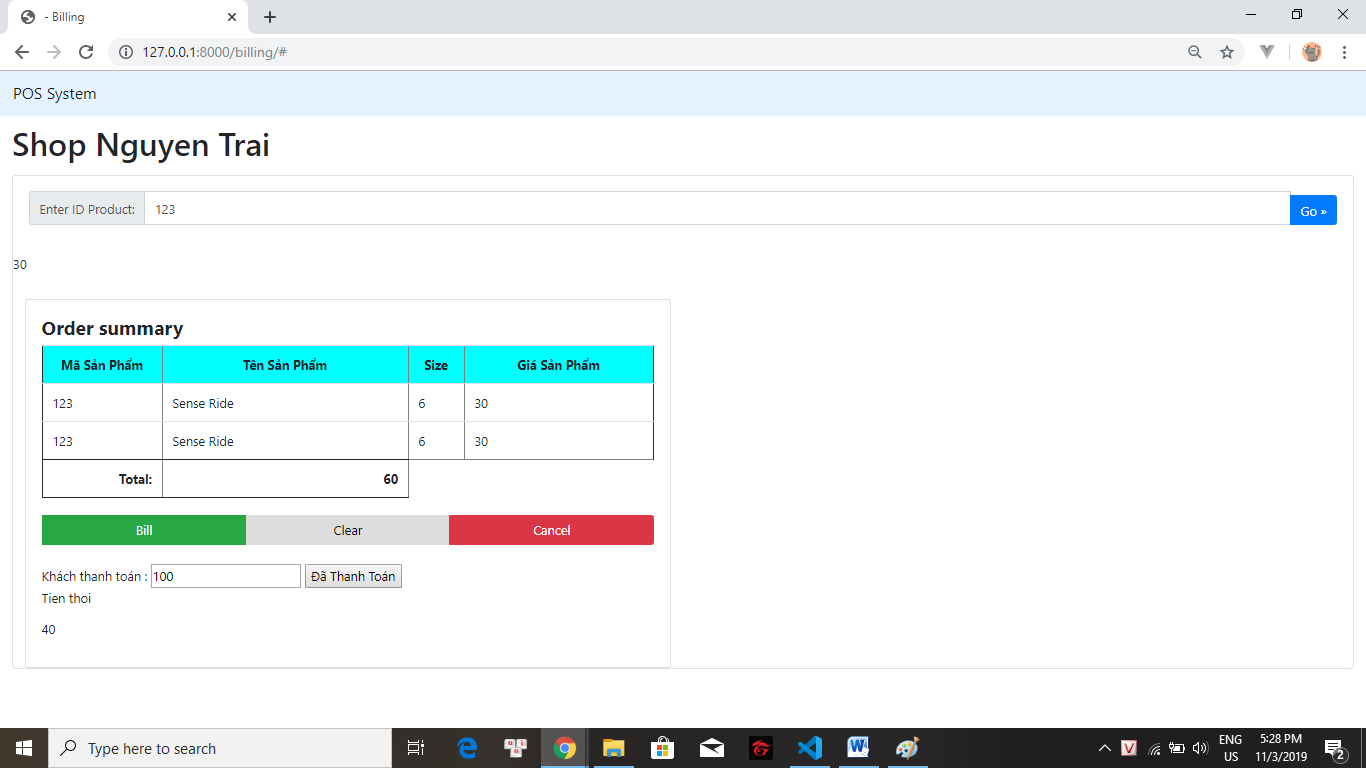
\includegraphics[scale = 0.5]{26.png}

Bước 5: Chốt hóa đơn bằng cách nhấn nút “Bill”. Nếu thanh toán thành công, trang thanh toán sẽ hiển thị “ Order Successful”, ngược lại sẽ hiển thị “Orer Failed” \\

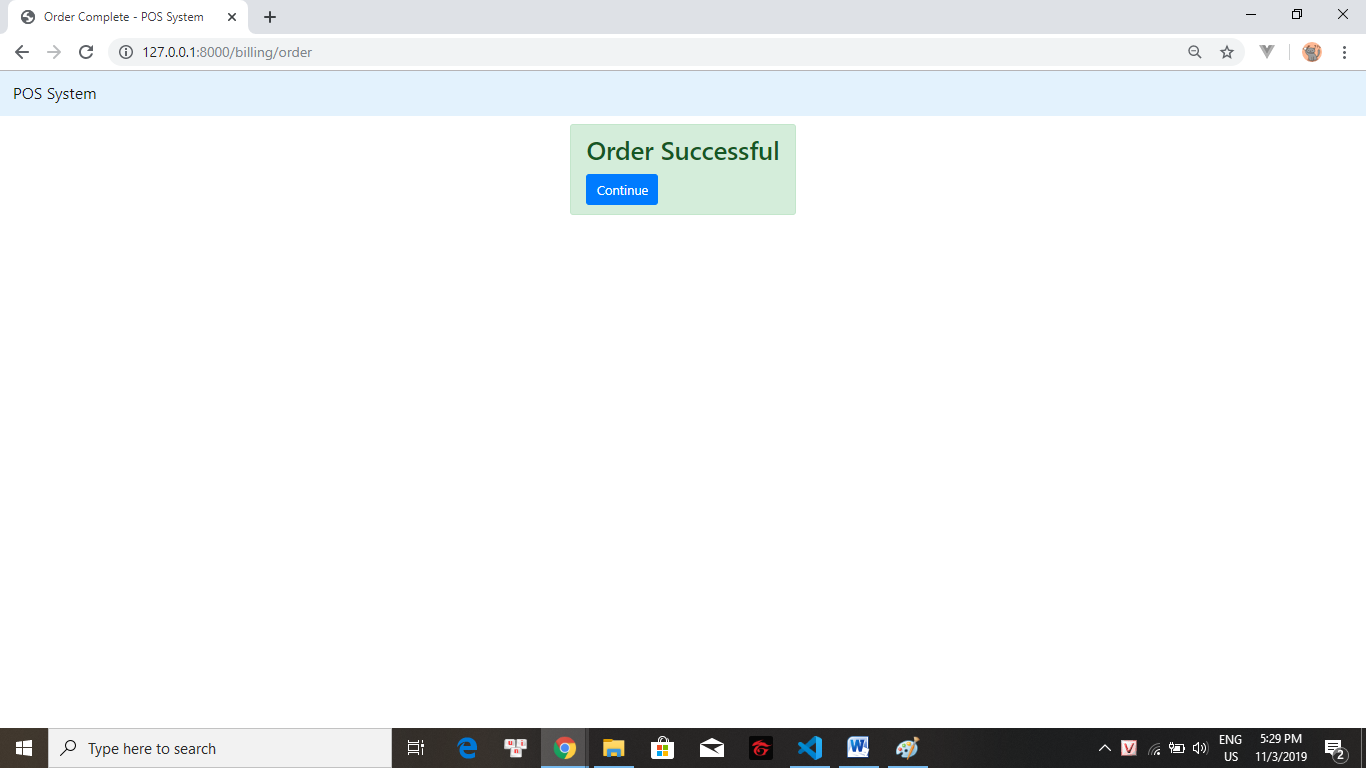
\includegraphics[scale = 0.5]{27.png}

\end{document}